\pdfoutput=1

\documentclass[11pt]{article}

\usepackage[final]{acl}

\usepackage{times}
\usepackage{latexsym}
\usepackage{amsmath} 
\usepackage{graphicx}
\usepackage{hyperref}
\usepackage{url}
\usepackage{amsfonts}
\usepackage{graphicx} 
\usepackage{multirow}
\usepackage{array}
\usepackage{caption}
\usepackage{xcolor}
\usepackage{booktabs}
\usepackage[T1]{fontenc}

\usepackage[utf8]{inputenc}

\usepackage{microtype}

\usepackage{inconsolata}

\usepackage{graphicx}
\newcommand{\hanjie}[1]{{\color{teal} [{\bf Hanjie}: #1]}}
\newcommand{\roy}[1]{{\color{blue} [{\bf Roy}: #1]}}
\newcommand{\cy}[1]{{\color{brown} [{\bf Chunyuan}: #1]}}
\title{Language Models are Symbolic Learners in Arithmetic}
\author{Chunyuan Deng$^1$ \quad Zhiqi Li$^{2}$ \quad Roy Xie$^3$ \quad Ruidi Chang$^1$ \quad Hanjie Chen$^{1}$ \\
$^1$Rice University \quad $^2$Georgia Tech \quad $^3$Duke University\\
\texttt{\{chunyuan.deng,hanjie\}@rice.edu} \\
}
\vspace{-2cm}
\begin{document}
\maketitle
\begin{abstract}
Large Language Models (LLMs) are thought to struggle with arithmetic learning due to the inherent differences between language modeling and numerical computation, but concrete evidence has been lacking. This work responds to this claim through a two-side experiment. We first investigate whether LLMs leverage partial products during arithmetic learning. We find that although LLMs can identify some partial products after learning, they fail to leverage them for arithmetic tasks, conversely. We then explore how LLMs approach arithmetic symbolically by breaking tasks into subgroups, hypothesizing that difficulties arise from subgroup complexity and selection. Our results show that when subgroup complexity is fixed, LLMs treat a collection of different arithmetic operations similarly. By analyzing position-level accuracy across different training sizes, we further observe that it follows a U-shaped pattern: LLMs quickly learn the easiest patterns at the first and last positions, while progressively learning the more difficult patterns in the middle positions. This suggests that LLMs select subgroup following an easy-to-hard paradigm during learning. Our work confirms that LLMs are pure symbolic learners in arithmetic tasks and underscores the importance of understanding them deeply through subgroup-level quantification. 
\end{abstract}
\section{Introduction}
Modern math benchmarks like MATH~\citep{hendrycks2021measuringmathematicalproblemsolving} and GSM8K~\citep{cobbe2021trainingverifierssolvemath} have been rapidly saturated due to the advancements of frontier language models like GPT-4o~\citep{openai2024gpt4technicalreport} and Claude~\citep{claude}. 
This trend is driving the assessment of these models toward more challenging tasks, such as Olympic Math. However, it has been observed that even the most advanced language models struggle with basic arithmetic, such as 5-digit multiplication~\citep{yang2023gptsolvemathematicalproblems}. This notable gap raises questions about the underlying mechanisms behind arithmetic in language models. And some hypothesize~\citep{boguraev2024modelsembracecommunicativenature} that this difficulty stems from the fact that mathematical calculation differs fundamentally from autoregressive language modeling.

Previous research on this topic has primarily focused on causal abstraction to identify model components such as key attention layers~\citep{stolfo-etal-2023-mechanistic} or attention heads~\citep{zhang2024interpretingimprovinglargelanguage} responsible for arithmetic learning.  While these studies provide valuable insights into the components involved in mathematical operations, they fall short of explaining why frontier models continue to struggle with certain arithmetic tasks. For instance, causal attribution reveals that the 14th attention head in the $19$th layer is responsible for the operation $37 + 14 = 51$. 
However, it cannot explain why the model handles $37 + 14$ successfully but fails on $37 \times 14$. This observation suggests that there is still room to explore arithmetic learning from alternative perspectives.
\begin{figure*}[t]
\vspace{-0.3cm}
\begin{center}
        \centering 
        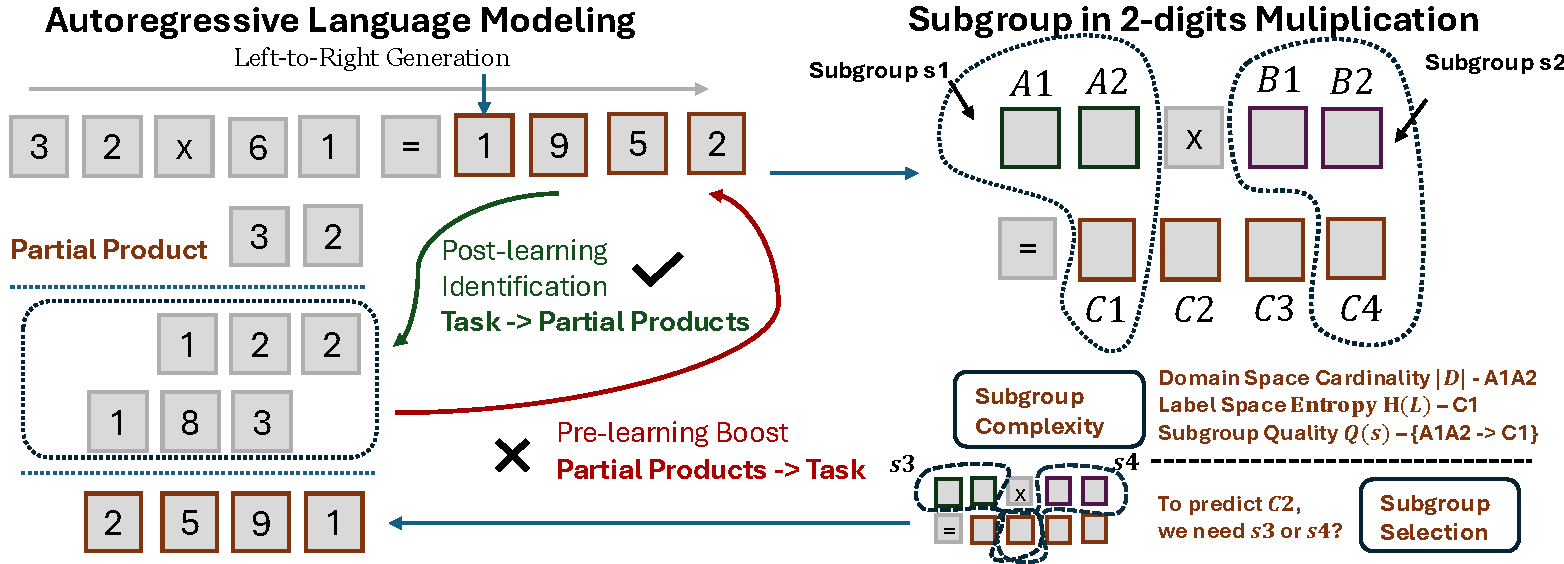
\includegraphics[width=\linewidth]{figure/intro.pdf}
        \caption{Fundamental structure of the paper. We begin by investigating partial products and proceed to a detailed examination at the subgroup level to understand the mechanism in a symbolic manner.}
        \label{fig:flowchart}
\end{center}
\vspace{-0.8cm}
\end{figure*}

To achieve this, we approach this problem from two sides (shown in Figure~\ref{fig:flowchart}). First, we examine whether LLMs leverage partial products in arithmetic learning tasks. Then we explore whether, and more importantly, \textit{how} LLMs handle arithmetic in a purely symbolic manner. Specifically, we decompose the task into subgroup level, hypothesizing the task can be understood through two aspects: subgroup complexity and subgroup selection.

For partial products, we considered four distinct methods for multiplication calculation: standard multiplication, repetitive addition, the lattice method, and Egyptian multiplication (detailed in~\S\ref{sec:his_mod_multi}), each generating distinct paths for partial product computation. We first fine-tune LLMs on multiplication tasks. After fine-tuning, models improved in identifying nearly all partial products, but explicit training on partial products did not enhance their ability to perform multiplications, instead. These findings suggest that large language models may not leverage partial products to perform arithmetic calculations. The increased ability to identify partial products seems to be a by-product of subgroup-level symbol learning rather than a mechanism the models inherently use for computation.

We then delve into a more fine-grained level by examining subgroups to understand their basic complexity. Subgroup complexity refers to the intrinsic complexity of the subgroup itself. We propose that this is related to the domain space cardinality $|\mathcal{D}|$, label space entropy $H(\mathcal{L})$, and subgroup quality $Q(s)$. Here, $|\mathcal{D}|$ represents the maximum size of training data, $H(\mathcal{L})$ represents the variability in the label space, and $Q(s)$ refers to how deterministically one subgroup can map from the domain to the label space. While $|\mathcal{D}|$, which strongly correlated with training size, is self-evident to influence learning, we will focus on label space entropy $H(\mathcal{L})$ first then discuss $Q(s)$ in the subgroup selection section. We observe influence of $H(\mathcal{L})$ by introducing perturbations to addition and multiplication by applying translation ($\Delta c$) and scaling ($\times \lambda$), while maintaining the total entropy the same across all output digits. Our findings show that LLMs have nearly the same accuracy across different perturbation magnitudes. Furthermore, when we intentionally reduce the entropy of the label space via modular operations, we observe an increase in accuracy as entropy decreases. These experiments confirm that label space entropy is an effective measure for quantifying task complexity and validates the hypothesis that LLMs operate as symbol-level pattern finders.

Subgroup selection refers to the process by which LLMs identify the correct subgroup during training, specifically by selecting the appropriate mapping between a token subset in the input domain and a corresponding token subset in the output label space. To investigate this, we curated four distinct training sets to analyze position-level accuracy throughout the learning process. Consistent patterns emerged: position-level accuracy exhibited a U-shaped curve, achieving near-perfect accuracy (close to $100\%$) at both the beginning and end of digits with high $Q(s)$, but dropping significantly (to below $10\%$) across the intermediate digits with low $Q(s)$. These results suggest that LLMs apply a selection mechanism driven by high-to-low subgroup quality, providing further evidence of their symbolic learning behavior.

Our work confirms that LLMs do not truly perform calculations in arithmetic learning. Instead, they approach it in a purely symbolic manner. We then provide a systematic framework to examine this mechanism from subgroup complexity and subgroup selection. Our research emphasizes the pivotal role of label space entropy in the convergence stage and the impact of subgroup quality on learning dynamics, highlighting the importance of deeply understanding arithmetic through subgroup-level quantification symbolically.
\section{Related Work}
\paragraph{Mathematical Learning in LLMs}
Mathematical reasoning has been a longstanding area of research in natural language processing (NLP)~\citep{kushman-etal-2014-learning,huang-etal-2016-well,wang-etal-2017-deep,thawani-etal-2021-representing,Sundaram2022WhyAN,guo2024learningpatternmatchingassaying}. With recent advances in LLM, numerous studies have sought to improve their mathematical reasoning abilities through various techniques, including data annealing~\citep{dubey2024llama3herdmodels}, continued pretraining~\citep{lewkowycz2022solving}, fine-tuning~\citep{Yue2023MAmmoTHBM,liu2023improvinglargelanguagemodel}, prompting~\citep{wei2023chainofthoughtpromptingelicitsreasoning,wang2023selfconsistencyimproveschainthought}, and inference-time computation~\citep{Zhou2023LanguageAT,wu2024mathchatconversetacklechallenging}. However, LLMs still face challenges with basic calculations and remain vulnerable to adversarial examples or perturbations, where minor changes in problems can result in incorrect answers~\citep{zhou2023mathattackattackinglargelanguage,xie2024adversarialmathwordproblem}. Most research on LLMs' mathematical reasoning focuses on math word problems, where natural language is involved in the questions \citep{hendrycks2021measuringmathematicalproblemsolving, cobbe2021trainingverifierssolvemath,Arora2023HaveLA,zhao2024financemath,zhao2024docmatheval}.
\paragraph{Arithmetic Learning in Transformer}
Several previous efforts have aimed to improve arithmetic learning in LLMs.~\citet{lee2023teachingarithmeticsmalltransformers} trained a 10.6M NanoGPT~\cite{karpathy2022nanoGPT} model to learn arithmetic by carefully curating the data format, explicitly expanding each step using a method termed Scratchpad, which achieved remarkable performance compared to GPT-2 XL~\citep{radford2019language}. ~\citet{yang2023gptsolvemathematicalproblems} fine-tuned MathGLM with a sufficient training dataset, demonstrating its capability to solve 5-digit multiplication. \citet{deng2023implicitchainthoughtreasoning,deng2024explicitcotimplicitcot} further advanced this field by internalizing the CoT process, hiding detailed steps in a scheduled manner, enabling GPT-2 small to solve 9-digit multiplication after multiple training runs. 

Research on understanding arithmetic primarily stems from the interpretability community. The core idea is to identify \textit{causal correlations} between model components and outputs. \citet{stolfo-etal-2023-mechanistic} identify key attention layers responsible for arithmetic learning using causal mediation analysis (CMA), a weight perturbation method that observes changes in output. Similarly, \citet{hanna2023doesgpt2computegreaterthan} and \citet{wu2024interpretabilityscaleidentifyingcausal} explore causal abstraction concepts at different model scales, specifically 0.1B and 7B parameters, respectively. More recently, \citet{zhang2024interpretingimprovinglargelanguage} employed an attention attribution to isolate a small subset of attention heads and fine-tune them for improved performance at a lower cost. While these studies have made progress in understanding how LMs perform arithmetic at a component level, there remains a gap in understanding the learning mechanisms from a purely symbolic perspective. Our research aims to contribute to this missing gap in a systematic manner.

\section{Preliminaries}
\label{sec:preliminaries}
In this section, we present the preliminaries of basic autoregressive language modeling, along with algebraic structure and arithmetic learning.

\paragraph{Autoregressive Language Modeling}
An autoregressive (AR) language model predicts the next token in a sequence based on the previously observed tokens. Formally, given a sequence of tokens $\mathbf{x} = \{x_1, x_2, \dots, x_T\}$, the probability of the sequence is decomposed using the chain rule of probability as:
\begin{equation}
    P(\mathbf{x}) = \prod_{t=1}^{T} P(x_t | x_1, x_2, \dots, x_{t-1}),
\end{equation}
where $P(x_t | x_1, x_2, \dots, x_{t-1})$ represents the conditional probability of token $x_t$ given all previous tokens. In autoregressive modeling, the next token is sampled from the conditional distribution $P(x_t | x_1, x_2, \dots, x_{t-1})$ until the end of the sequence is reached.

\paragraph{Algebraic Structure}

In our setting, we employ the algebraic structure known as a \textit{ring}, which provides a formal framework for the arithmetic operations of \textit{addition} and \textit{multiplication}. A ring $(R, +, \cdot)$ is defined by:

\begin{itemize}
    \item A set $R$ (domain) of elements. Specifically, the domain $R$ in our task is the set of integers $\mathbb{Z}$.
    \item Two binary operations, addition and multiplication $f(a,b)=c : R \times R \to R$. Specifically, we use $A_1A_2 + B_1B_2 = C_1C_2$ to represent 2-digit addition. We use $A_1A_2 \times B_1B_2 = C_1C_2C_3C_4$ to represent 2-digit multiplication.
\end{itemize}

In our case, for all $a, b \in R$, there exists a unique element $a + b \in R$, representing the sum of $a$ and $b$. Similarly, there exists a unique element $a \cdot b \in R$, representing the product of $a$ and $b$.


\paragraph{Arithmetic Learning}
\label{section:arithmetiC_learning_def}
Let $\mathcal{M}$ denote a pretrained autoregressive language model with weights $\mathbf{w}$. We define an arithmetic task $\mathcal{T}$ as a function learning problem where the goal is to predict numerical outputs based on arithmetic expressions. The training dataset for this task is given by:
\[
\mathbb{D}_{\text{train}} = \{(a^{(k)}, b^{(k)}, c^{(k)}\}_{k=1}^{N}
\]
where $c^{(k)} = f(a^{(k)}, b^{(k)})$ and $f(\cdot)$ represents a binary operator, $N$ denotes the number of data points. In this context, $a^{(k)}$ and $b^{(k)}$ are input operands, and $c^{(k)}$ is the corresponding output, which is computed using the operator $f$ (e.g., addition, multiplication, etc.)


\section{Experiment Setup}
In this section, we will detail our experiment setup. Unless otherwise specified, the same setup will be used in the following section.

\paragraph{Domain}
We select addition and multiplication as the fundamental operations for our experiments following previous work~\citep{lee2023teachingarithmeticsmalltransformers,deng2023implicitchainthoughtreasoning,deng2024explicitcotimplicitcot}.
\paragraph{Model}
To investigate arithmetic learning at scale, we selected two open-source LLMs, Gemma-2-2B~\citep{gemmateam2024gemma2improvingopen} and Llama-3.1-8B~\citep{dubey2024llama3herdmodels}. Both models are top performers in their respective categories and excel at language-related tasks. We did not choose  GPT-4o~\citep{openai2024gpt4technicalreport} or other proprietary LLMs due to concerns that they may internally integrate function calling (e.g., invoking APIs or executing Python programs), which could affect the experimental setup. Training details is included at Appendix~\ref{appendix:training-detail}.

\paragraph{Conventional Data Format}
We directly train the model to predict the output (e.g., $130$) given the input operands and the operator (e.g., $13 \times 10$). e add one space between each digit to ensure tokens are split into individual digits We do not consider chain-of-thought (CoT)~\citep{wei2023chainofthoughtpromptingelicitsreasoning} or other prompting strategies to enforce the model to focus on arithmetic learning. We include ablations with respect to data format in Appendix~\ref{appendix:datA_format}.

\section{Are Large Language Models Implicit Calculators?}
In this section, we explore whether LLMs utilize partial products to enhance their arithmetic calculation capabilities, particularly in the context of \textit{multiplication}. It is important to note that while multiplication is well-defined mathematically, the process of multiplication calculation is not limited to traditional methods defined in textbook. Thus, examining only one calculation method presents a flawed experimental design that is vulnerable to exploitation. We selected four calculation methods that are representative to cover the major approaches to multiplication.
\subsection{Historical and Modern Multiplication}
\label{sec:his_mod_multi}
In terms of multiplication, four different calculation methods are most representative from history to now: Standard Multiplication, Repetitive Addition, Lattice Method, 
and Egyptian Multiplication.
\paragraph{M1: Standard Multiplication}
In standard multiplication, we multiply each digit of one number by each digit of the other number, and then sum the results appropriately:
\begin{align*}
12 \times 34 &= 12 \times (30 + 4) = 12 \times 30 + 12 \times 4 \\
&= 360 + 48 = 408
\end{align*}
\paragraph{M2: Repetitive Addition}
Multiplication can be interpreted as repeated addition. For \(12 \times 34\), we add \(12\) thirty-four times:
\begin{align*}
12 \times 34 &= 12 + 12 + 12 + \dots + 12 \quad (\text{34 times}) \\
&= 408
\end{align*}
\paragraph{M3: Lattice Method}
In the lattice method (or grid method), we place the numbers along the top and side of a grid, perform single-digit multiplications, and then sum along the diagonals:
\begin{align*}
12 \times 34 = 10 \times 30 &= 300 \\
10 \times 4 &= 40 \\
2 \times 30 &= 60 \\
2 \times 4 &= 8 \\
\text{Summing the results:} &\ 300 + 40 + 60 + 8 = 408
\end{align*}
\paragraph{M4: Egyptian Multiplication}
Egyptian multiplication computes the product by doubling the multiplicand and adding the results corresponding to the powers of two that sum to the multiplier. For \(12 \times 34\):
\begin{align*}
12 \times 34 = 12 \times 1 &= 12 \\
12 \times 2 &= \mathbf{24} \\
12 \times 4 &= 48 \\
12 \times 8 &= 96 \\
12 \times 16 &= 192 \\
12 \times 32 &= \mathbf{384} \\
\text{Summing the selected results:} &\ 24 + 384 = 408
\end{align*}
Since \(34 = 2 + 32\), we select the results for \(12 \times 16\) and \(12 \times 8\), and summing these gives the final product.
\begin{table*}[t]
\vspace{-0.5cm}
\vspace{-0.2cm}

\centering
\small
\resizebox{\textwidth}{!}{
\begin{tabular}{lcccccccc}
\toprule
& \multicolumn{4}{c}{Gemma-2-2B} & \multicolumn{4}{c}{Llama-3.1-8B} \\
\cmidrule(lr){2-5} \cmidrule(lr){6-9}
& Standard & Lattice & Repetitive  & Egyptian & Standard & Lattice & Repetitive  & Egyptian \\
\midrule
Task $\rightarrow$ Partial P. & $+4.1\%$ & $+6.8\%$ & $-29.0\%$ & $+3.6\%$ & $+40.6\%$ & $+40.8\%$ & $-59.0\%$ & $+29.6\%$ \\
Partial P. $\rightarrow$ Task & $-6.1\%$ & $-10.7\%$ & $-20.3\%$ & $-9.6\%$ & $-3.7\%$ & $-0.2\%$ & $-0.9\%$ & $-2.7\%$ \\
\bottomrule
\end{tabular}}
\caption{Inductive and deductive accuracy difference $\Delta$.}
\label{tab:partial-products}
\end{table*}

\subsection{Examining Partial Product in Arithmetic Learning}
To investigate whether LLMs generate partial products during arithmetic learning, we employ a set of diagnostic tasks as an approach to trace. We fine-tune Gemma-2-2B and Llama-3.1-8B on two-digit multiplication, observing changes in accuracy on diagnostic sets before and after fine-tuning (Task $\rightarrow$ Partial Products). Subsequently, we fine-tune the LLMs on these diagnostic sets and examine how their accuracy on the multiplication task changes (Partial Products $\rightarrow$ Task).
\begin{table}[!h]
\vspace{-0.2cm}
\centering
\small
\resizebox{0.49\textwidth}{!}{
\begin{tabular}{lccc}
\toprule
Method & \multicolumn{1}{c}{Diagnostic Sets} \\
\midrule
Standard Multiplication & $\mathcal{P_{\text{std}}} = \{{ A_1 \times B_1B_2,  A_2 \times B_1B_2, B_1 \times A_1A_2, B_2 \times A_1A_2 }\}$\\
\vspace{+0.05cm}
Repetitive Addition  & $\mathcal{P_{\text{ra}}} = \{{ \sum_{i=1}^{B_1B_2} A_1A_2, \sum_{i=1}^{A_1A_2} B_1B_2 }\}$ \\
Lattice Method  & $\mathcal{P_{\text{lattice}}} = \{{ A_10 \times B_10,A_10 \times B_2,A_2 \times B_10,A_2 \times B_2}\}$  \\
Egyptian Multiplication  & $\mathcal{P_{\text{egyptian}}} = \{{ 2^k \times A_1A_2 \mid k \in 0, 1, \ldots, \lfloor \log_{2}(B_1B_2) \rfloor}\}$\\
\bottomrule
\end{tabular}}
\caption{Diagnostic sets with four calculation methods.}
\label{tab:diagnostic-sets}
\vspace{-0.2cm}
\end{table}

We probe language models' partial product in four different directions. As shown in Table~\ref{tab:diagnostic-sets}, for a task formatting like $A_1A_2 \times B_1B_2 = C_1C_2C_3C_4 $, we would generate diagnostic test for each algorithm (detailed derivation in Appendix~\ref{appendix:diagnostiC_sets}).



\paragraph{Accuracy on Identifying Partial Products}
According to the results in Figure~\ref{fig:partial_products}, we found that standard multiplication, the lattice method, and the Egyptian method significantly improved in identifying partial products after fine-tuning, with gains of +$17.45\%$, +$18.35\%$, and +$10.45\%$, respectively. However, for repetitive addition tasks, LLMs failed to identify partial products, achieving an accuracy of only about $5\%$ after fine-tuning.
\begin{figure}[ht]
    \centering
    \includegraphics[width=0.98\linewidth]{figure/metriC_comparison_new.pdf}
    \caption{Partial products identification accuracy before and after fine-tuning on tasks. Scores are reported on average of Gemma-2-2B and Llama-3.1-8B.}\label{fig:partial_products}
    \vspace{-0.4cm}
\end{figure}
\paragraph{A Deeper Look into Calculations}
Do the results showing increased accuracy across three paths really imply that partial products are used in arithmetic learning? We have two arguments against this interpretation. First, if LLMs genuinely use partial products to learn arithmetic, it is likely that they only use one calculation path at a time. Thus, the simultaneous improvement across three paths (standard, lattice, and Egyptian) is unusual. Second, if LLMs employ a specific path to compute partial products, this process should be demonstrated as bidirectional. Specifically, LLMs fine-tuned on a task should be able to identify partial products (inductive), and conversely, mastering partial products should enhance task learning (deductive). However, we currently have results for only one direction, lacking evidence for the other. Therefore, we extend our experiments to another direction.
\paragraph{Accuracy on Identifying Tasks}
We fine-tune two LLMs on diagnostic sets and present the results of identifying tasks before and after fine-tuning in Table~\ref{tab:partial-products}. Our findings reveal that,
fine-tuning specifically on partial products does not enhance task learning. Instead, it results in a performance drop across all four calculation paths for both models. This indicates that pre-learning partial products does not aid in arithmetic learning. The improved ability to recognize partial products appears to stem from the symbol learning process (note that the standard partial product $A_1 \times B_1B_2$ is a sub-portion of $A_1A_2 \times B_1B_2$, similar to lattice and Egyptian methods) rather than being an intrinsic computational method used by the models.

\section{Are Language Models Symbolic Observers?}
An intuitive alternative for explaining increasing performance from inductive tasks (Task $\rightarrow$ Partial Products) is to treat LLMs as subgroup-level symbol observers, which aligns with the intrinsic properties of language modeling. Notably, the standard multiplication, lattice method, and Egyptian methods share a similar structure, where their partial product sets form token-level subgroups within the tasks. This observation naturally leads us to explore this idea further.
\subsection{Define Subgroup in Token Level}
\label{sec:subgroup_def}
We first define subgroup in this section. Arithmetic learning involves a training set $\mathbb{D}_{\text{train}}=\{(a^{(k)}, b^{(k)}), c^{(k)} \}_{k=1}^{N}$ \text{where} $c^{(k)} = f(a^{(k)}, b^{(k)})$ and $f(\cdot)$ represents a binary operator, $N$ is the number of dataset. In \( n \)-digit arithmetic learning, \( a^{(k)} \) and \( b^{(k)} \) can be regarded as different values taken by random variable sequences, \( \{A_i\}_{i=1}^n \) and \( \{B_i\}_{i=1}^n \), respectively. The random variables \( A_i\) and \(B_i\) all follow a discrete uniform distribution \( P(X = x) = \frac{1}{10}, x = 0,1,...,9 \).  \( c^{(k)} \) can be regarded as different values taken by random variable sequence \( \{C_i\}_{i=1}^{m} \), where the random variables  \( C_i, i=1,...,m\) has a joint distribution given by: 
\begin{align*}
&I_{\{f(a,b) = c\}} P(\{A_i\}_{i=1}^n = a) P(\{B_i\}_{i=1}^n = b)    
\end{align*}
where $I_{\{f(a,b) = c\}}$ is indicator function equals 1 if the condition $f(a,b) = c$ holds true, and 0 otherwise. 

\paragraph{Definition 1 (Subgroup):}
For \( n \)-digit arithmetic, a subgroup $s$ is defined as any element of the set \( \mathbb{S}_n \):
\[
\scalebox{0.75}{$
s \in \mathbb{S}_n = \{((\mathbb{A}, \mathbb{B}), \mathbb{C}) \mid \mathbb{A} \subseteq \{A_i\}_{i=1}^n, \mathbb{B} \subseteq \{B_i\}_{i=1}^n, \mathbb{C} \subseteq \{C_i\}_{i=1}^{m}\}
$}
\]
where \( \mathbb{A} \), \( \mathbb{B} \) and \( \mathbb{C} \) can be any subportion of random variable sequences \(\{A_i\}_{i=1}^n\), \( \{B_i\}_{i=1}^n \) and \(\{C_i\}_{i=1}^n\), respectively. Specifically, we use $s_i \in \mathbb{S}_n$ to denote subgroups in $i$-th prediction for $C_i$.

\paragraph{Definition 2 (Subgroup Space):}
For any subgroup $s = ((\mathbb{A}, \mathbb{B}), \mathbb{C}) \in \mathbb{S}_n$, we have:
\vspace{-0.2cm}
\begin{itemize}
    \item Domain Space: $\mathcal{D}_s = \{(\{a\}_{k=1}^{|\mathbb{A}|}, \{b\}_{k=1}^{|\mathbb{B}|}) \mid P(\mathbb{A}=\{a\}_{k=1}^{|\mathbb{A}|})>0,P(\mathbb{B}=\{b\}_{k=1}^{|\mathbb{B}|})>0\}$. The size of domain space or cardinality
 is annotated as $|\mathcal{D}_s|$.
 \vspace{-0.4cm}
    \item Label Space: $\mathcal{L}_s = \{\{c\}_{k=1}^{|\mathbb{C}|} \mid P(\mathbb{C}=\{c\}_{k=1}^{|\mathbb{C}|})>0\}$.  The size of label space is annotated as $|\mathcal{L}_s|$.
\vspace{-0.2cm}
\end{itemize}
The entropy of label space is given by:
\[
H(\mathcal{L}_s) = -\sum_{y \in \mathcal{L}_s}P(\mathbb{C}=y)  \log_2 P(\mathbb{C}=y)
\vspace{-0.2cm}
\]
\begin{table*}[ht]
\vspace{-1.2cm}
\centering
\small
\resizebox{\textwidth}{!}{
\begin{tabular}{llccccccc}
\toprule
& &\multicolumn{1}{c}{$C_1$} & \multicolumn{1}{c}{$C_2$}& \multicolumn{1}{c}{$C_3$}& \multicolumn{1}{c}{$C_4$}&\multicolumn{1}{c}{$C_5$} &\multicolumn{2}{c}{$\{C_i\}_{i=1}^{n}$} \\
 \cmidrule(lr){8-9} 
Task & Format & $H(\mathcal{L})$ & $H(\mathcal{L})$ &  $H(\mathcal{L})$ & $H(\mathcal{L})$ & $H(\mathcal{L})$ & $|\mathcal{L}|$ & $H(\mathcal{L})$ \\
\midrule
$f(a,b) = a+b$ & $A_1A_2+B_1B_2=C_1C_2C_3$ & $0.9710$ & $3.3215$ & $3.3219$ & $-$ & $-$ &$179$ &$7.2130$\\
$f(a,b) = a+b+1$ & $A_1A_2+B_1B_2=C_1C_2C_3$  & $0.9649$ & $3.3215$ & $3.3219$ & $-$ & $-$ &$179$ &$7.2130$\\
$f(a,b) = a+b+15$ & $A_1A_2+B_1B_2=C_1C_2C_3$ & $0.9280$ & $3.3214$ & $3.3219$ & $-$ & $-$ &$179$ &$7.2130$ \\
$f(a,b) = a+b+115$ & $A_1A_2+B_1B_2=C_1C_2C_3$ & $0.9280$ & $3.3214$ & $3.3219$ & $-$ & $-$ &$179$ &$7.2130$ \\
$f(a,b) = (a+b) \: mod \: 100$ & $A_1A_2+B_1B_2=C_1C_2$  & $3.3214$ & $3.3219$ & $-$ & $-$ & $-$ & $100$ & $6.6432$ \\
$f(a,b) = (a+b) \: mod \: 50 $ & $A_1A_2+B_1B_2=C_1C_2$ & $2.3217$ & $3.3219$ & $-$ & $-$ & $-$ & $50$ & $5.6436$   \\
$f(a,b) = (a+b) \: mod \: 10 $ & $A_1A_2+B_1B_2=C_1$ & $3.3219$ & $-$ & $-$ & $-$ & $-$ & $10$ & $3.3219$  \\
\midrule
$f(a,b) = a \times b$ & $A_1A_2 \times B_1B_2=C_1C_2C_3C_4$  & $2.8979$ & $3.3215$ & $3.3160$ & $3.0340$ & $-$ & $2621$ &$11.1172$\\
$f(a,b) = a \times b \times 2$ & $A_1A_2 \times B_1B_2=C_1C_2C_3C_4C_5$ & $0.6873$ & $3.2173$ & $3.3215$ & $3.2964$ & $2.2227$ & $2621$ &$11.1172$ \\
$f(a,b) = a \times b \times 4 $& $A_1A_2 \times B_1B_2=C_1C_2C_3C_4C_5$ & $1.6030$ & $3.3020$ & $3.3204$ & $3.2234$ & $2.2227$ & $2621$ &$11.1172$\\
$f(a,b) = a \times b \times 8$ & $A_1A_2 \times B_1B_2=C_1C_2C_3C_4C_5$  & $2.5811$ & $3.3202$ & $3.3151$ & $3.2235$ & $2.2227$ & $2621$ &$11.1172$\\
$f(a,b) = (a \times b) \: mod \: 100$ & $A_1A_2 \times B_1B_2=C_1C_2$   & $3.3160$ & $3.0340$ & $-$ & $-$ & $-$ & $100$ &$6.2912$ \\
$f(a,b) = (a \times b) \: mod \: 50 $ & $A_1A_2 \times B_1B_2=C_1C_2$  & $2.3210$ & $3.0340$ & $-$ & $-$ & $-$ & $50$ &$5.3494$ \\
$f(a,b) = (a \times b) \: mod \: 10 $ & $A_1A_2 \times B_1B_2=C_1$  & $3.0340$ & $-$ & $-$ & $-$ & $-$ & $10$ &$3.0340$ \\
\bottomrule
\end{tabular}}
\caption{Label space statistics with different rule perturbations. $H(\mathcal{L})$ represents the entropy of the label space, and $|\mathcal{L}|$ is the size of the label space. $\{C_j\}_{i=1}^{n}$ represents all positions in output digits.}
\label{tab:subgroup-space}
\vspace{-0.4cm}
\end{table*}
\subsection{Difficulty in Arithmetic Learning: A Well-educated Hypothesis}
\label{sec:difficulty}
We propose the following hypothesis:
For an $n$-digit arithmetic task requiring $m$ predictions, the overall difficulty $\zeta$ is related to:
\begin{equation}
\zeta \propto \hat h^m
\end{equation}
where $\hat h=\prod_{i=1}^{m} h(s_i)^\frac{1}{m}$ represents the geometric average difficulty of an individual prediction, with $s_i \in \mathbb{S}_n$ denoting subgroup selection for the $i$-th prediction, and $h(\cdot)$ representing the subgroup complexity evaluation function.

\textbf{Subgroup Complexity ($h(\cdot)$):} This represents the most basic difficulty in arithmetic learning. It captures the inherent difficulty in the structure of the arithmetic learning tasks. We believe that the complexity on subgroup is strongly correlated with the property on that subgroup space:
\begin{itemize}

    \item \textit{Domain Space Cardinality \( |\mathcal{D}| \)}: The size of the domain space \( |\mathcal{D}| \) determines how many data points are available for learning a pattern. If the label space is fixed, a larger domain space generally leads to improved learning outcomes.

    \item \textit{Label Space Entropy \( H(\mathcal{L}) \)}: Label space entropy \( H(\mathcal{L}) \) is also a critical factor in learning, as a low-entropy label space often leads to higher predictability.
    \item \textit{Subgroup Quality $Q$}: For any subgroup \( s=((\mathbb{A},\mathbb{B}),\mathbb{C}) \in S_n \),
 \begin{align}
 \vspace{-0.2cm}
    Q(s) &=\max_{g \in \Omega_s} \sum_{a'=\{a\}_{k=1}^{|\mathbb{A}|}} \sum_{b'=\{b\}_{k=1}^{|\mathbb{B}|}} \sum_{c'=\{c\}_{k=1}^{|\mathbb{C}|}}\notag\\
    & P_s^f(a',b',c') P_s^p(g,a',b',c')
\vspace{-0.2cm}
\end{align}
    where \(\Omega_s: \mathcal{D}_s \to \Theta(\mathcal{L}_s)\) represents a function space mapping from \(\mathcal{D}_s\) to \(\Theta(\mathcal{L}_s)\), and \(\Theta(\mathcal{L}_s)\) denotes the space of random variables taking values in \(\mathcal{L}_s\).  Here, \( P_s^p(g, a',b',c') = P(g(a',b') = c') \) represents the probability that the function \( g \) maps \( (a',b') \) to \( c' \), and \( P_s^f(a', b', c') \) represents the probability that  \( \mathbb{A} = a' \), \( \mathbb{B} = b' \) and \( \mathbb{C} = c' \), hold simultaneously in arithmetic tasks. Thus, \( Q(s) \) measures the maximum possible probability of predicting the value of \( \mathbb{C} \) that is consistent with the values in the dataset from the values of \( (\mathbb{A}, \mathbb{B}) \).
\end{itemize}
\textbf{Subgroup Selection ($s_i$):} $s_i \in \mathbb{S}n$ represents the subgroup selection for the $i$-th prediction. When LLMs predict the token in the $i$-th position, they must select subgroups that include $C_i$ to align with the underlying pattern. This reflects the \textbf{learning dynamics} of language models in arithmetic tasks, abstractly linked to their decision-making and selection processes. As discussed in \S\ref{sec:subgroup-selection}, LLMs seem to initially select the subgroup $s_i$ with high quality $Q_{high}(s_i)$, progressing to lower quality $Q_{low}(s_i)$ (easy-to-hard) during learning.

\subsection{Subgroup Complexity: Label Space Matters in the Final Stage }
\label{sec:subgroup-complexity}
 In this section, we discuss subgroup complexity in arithmetic learning. The domain space cardinality $|\mathcal{D}|$ represents the number of training data available, which is an obvious factor influencing learning. Subgroup quality $Q(s)$ will be detailed in \S\ref{sec:subgroup-selection}. Thus, we primarily focus on \textit{label space entropy} $H(\mathcal{L})$ in this section.

\paragraph{Rule Perturbation}
We first deliberately perturb the rules to observe whether these changes affect task difficulty for LLMs. We consider addition $ f(a,b) = a + b$ and multiplication $ f(a,b) = a \times b $ as our baselines. For addition, the perturbation is defined as $ f(a,b) = a + b + \Delta c $, where $ \Delta c = 1, 15, 115 $ corresponds to perturbations at different position with different magnitudes. For multiplication, the perturbation is defined as $ f(a,b) = a \times b \times \lambda $, where $ \lambda = 2, 4, 8 $ following similar reasons above. Additionally, we incorporate modular addition and multiplication as further perturbations. Table~\ref{tab:subgroup-space} showcases the basic change for label space entropy after applying perturbations. We then fine-tune Gemma-2-2B and Llama-3.1-8B using different perturbation rules to observe how well these large language models can be influenced from such perturbations in learning.
\paragraph{Results}
The results in Table~\ref{tab:subgroup-space-results} demonstrate that across two different rule perturbation methods and three distinct setups, both Gemma-2-2B and Llama-3.1-8B yield consistent outcomes. While calculating $13 \times 27 = 2808$ may seem counterintuitive, LLMs handle this arithmetic same as $13 \times 27 = 351$ when the label space entropy $H(\mathcal{L})$ are fixed. 
\begin{table}[ht]
\vspace{-0.26cm}
\centering
\small
\resizebox{0.5\textwidth}{!}{
\begin{tabular}{lcc}
\toprule
& \multicolumn{1}{c}{Gemma-2-2B} & \multicolumn{1}{c}{Llama-3.1-8B} \\
\midrule
$f(a,b) = a+b$ & $-$ & $-$\\
$f(a,b) = a+b+1$ & $-0.1\%$ & $-0.1\%$ \\
$f(a,b) = a+b+15$ & $-0.9\%$ & $+0.1\%$ \\
$f(a,b) = a+b+115$ & $-1.4\%$ & $+0.7\%$ \\
\midrule
$f(a,b) = (a+b) \: mod \: 100$ & $+10.1\%$ & $+3.7\%$ \\
$f(a,b) = (a+b) \: mod \: 50$& $+13.1\%$ & $+6.7\%$ \\
$f(a,b) = (a+b) \: mod \: 10$& $+26.1\%$ & $+13.7\%$ \\
\midrule
$f(a,b) = a \times b$ & $-$ & $-$\\
$f(a,b) = a \times b \times 2$& $-1.1\%$ & $-2.7\%$ \\
$f(a,b) = a \times b \times 4$& $-1.7\%$ & $+0.7\%$ \\
$f(a,b) = a \times b \times 8$ & $+0.2\%$ & $-3.7\%$ \\
\midrule
$f(a,b) = (a \times b) \: mod \: 100$ & $+7.1\%$ & $+3.8\%$\\
$f(a,b) = (a \times b) \: mod \: 50$ & $+12.1\%$ & $+5.3\%$ \\
$f(a,b) = (a \times b) \: mod \: 10$ & $+18.9\%$ & $+10.7\%$ \\
\bottomrule
\end{tabular}}
\caption{Test Accuracy difference $\Delta$ on perturbed addition and multiplication.}
\label{tab:subgroup-space-results}
\vspace{-0.3cm}
\end{table}

 Regarding modular addition and multiplication with different modulus numbers, we find that decreasing the size of the entropy leads to performance improvements in both cases. These results highlight that an arithmetic task with low variability in the label space is more learnable. Together, these two observations reinforce the notion that LLMs are not performing traditional calculations but are instead functioning as sophisticated symbolic observers within the token space.
 \begin{figure*}[t]
\vspace{-0.4cm}
    \centering
    \hspace{-0.4cm}
    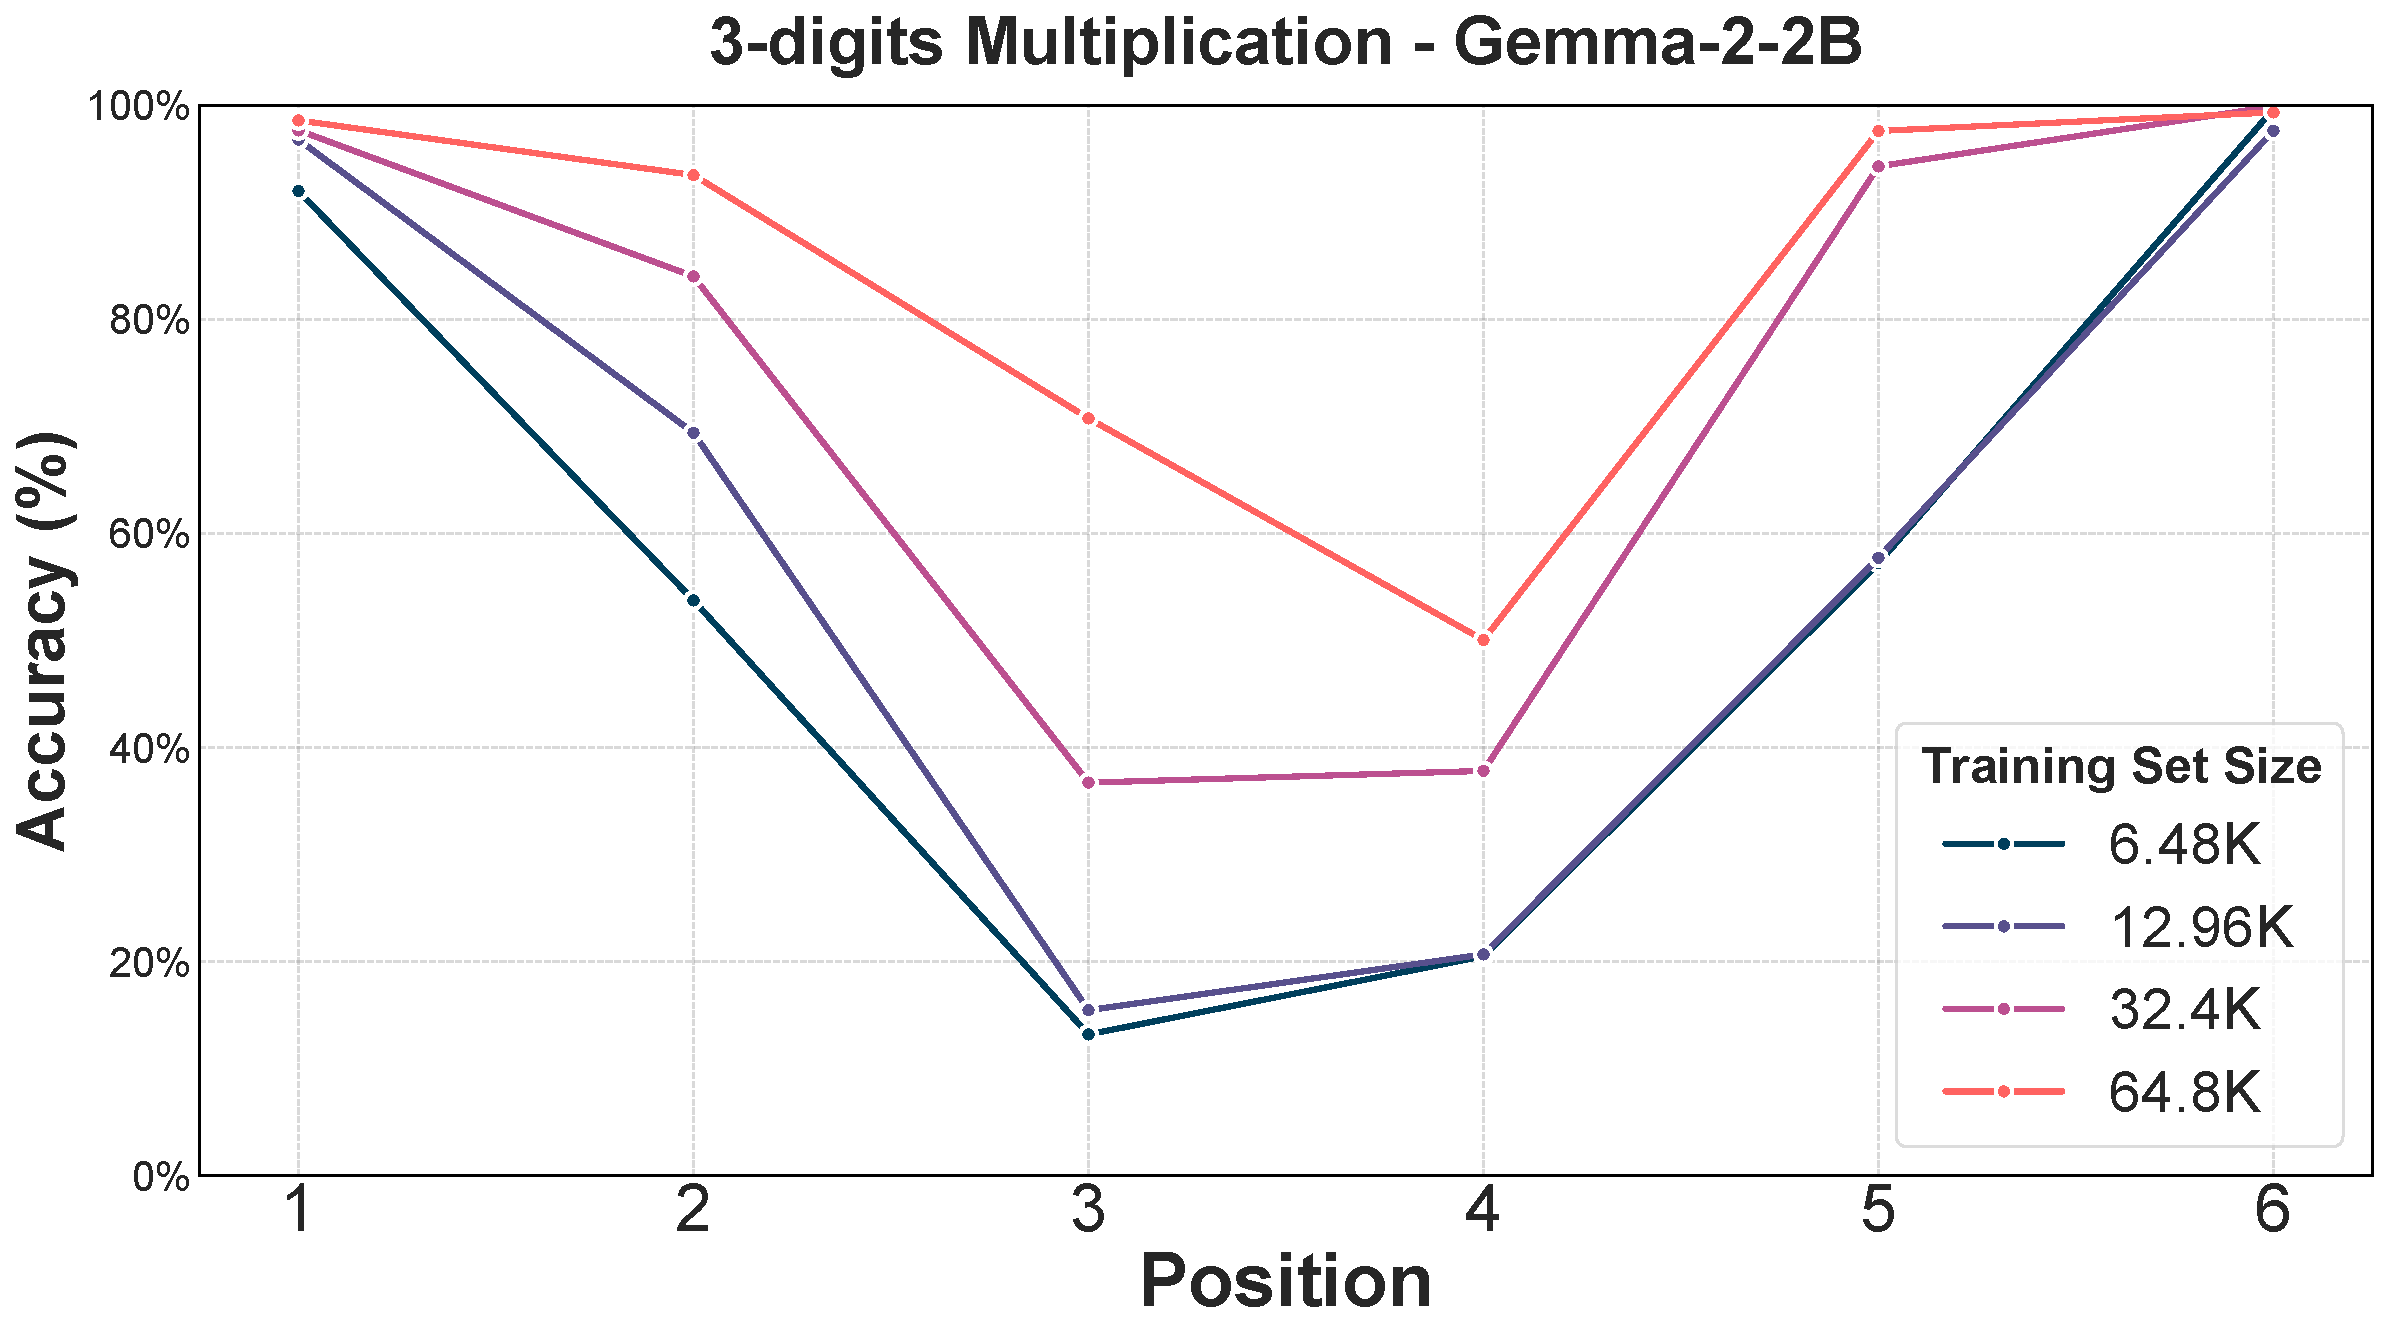
\includegraphics[width=0.33\linewidth]{figure/3x3_position_accuracy_chart-gemma.pdf}
    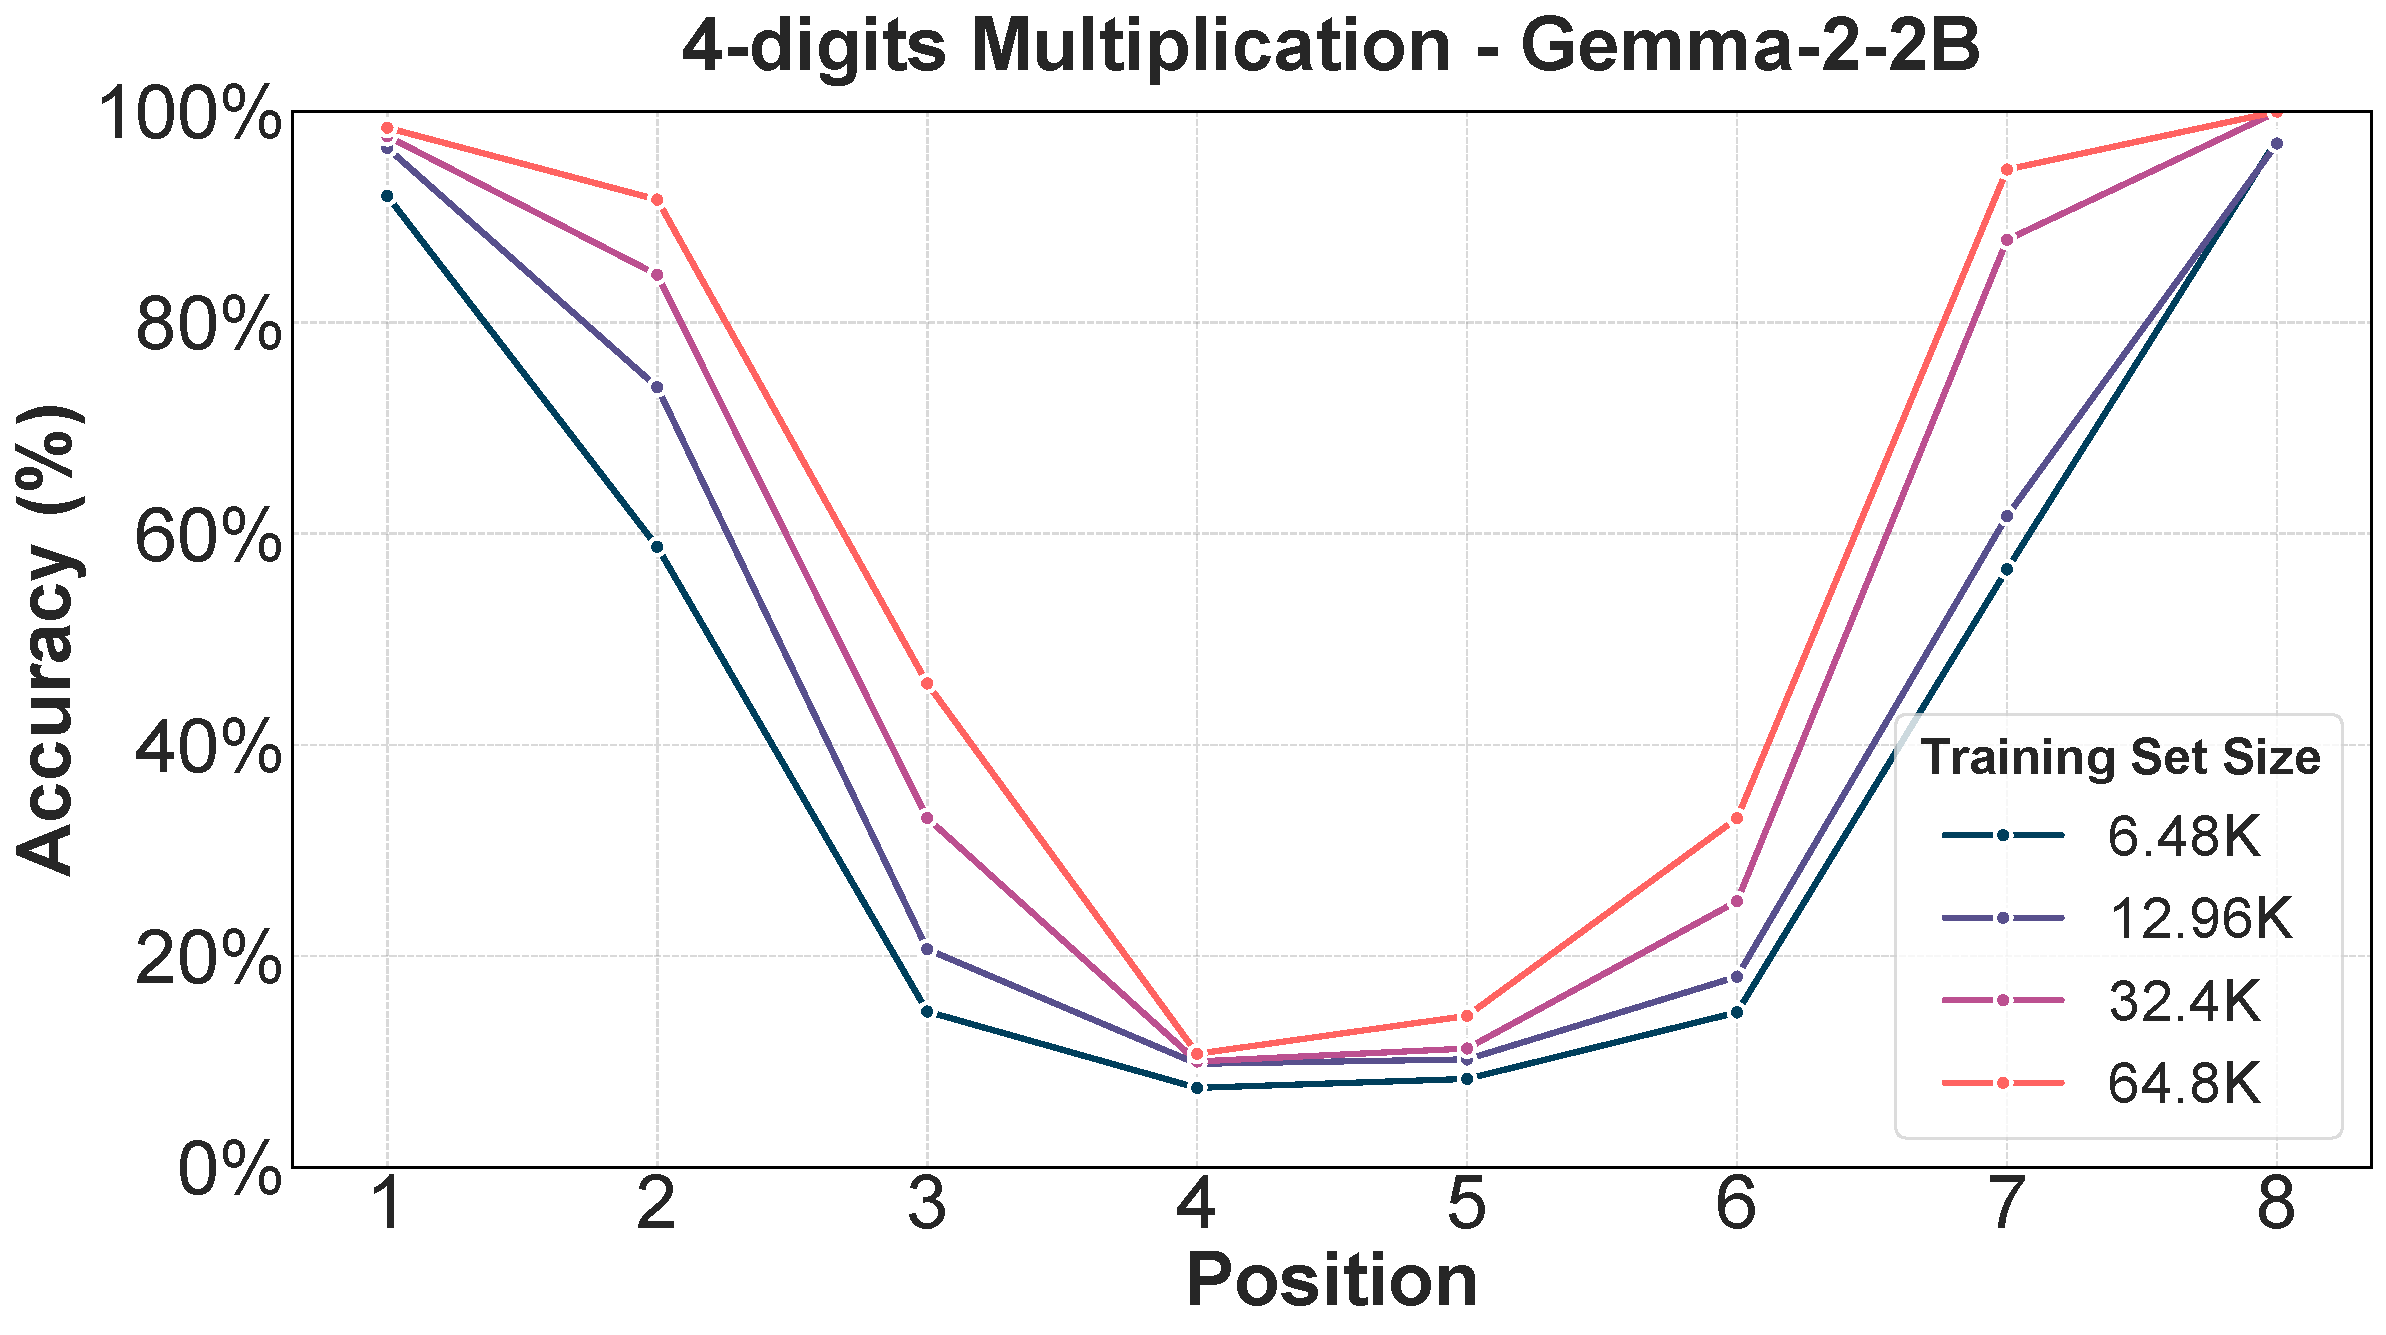
\includegraphics[width=0.33\linewidth]{figure/4x4_position_accuracy_chart-gemma.pdf}
    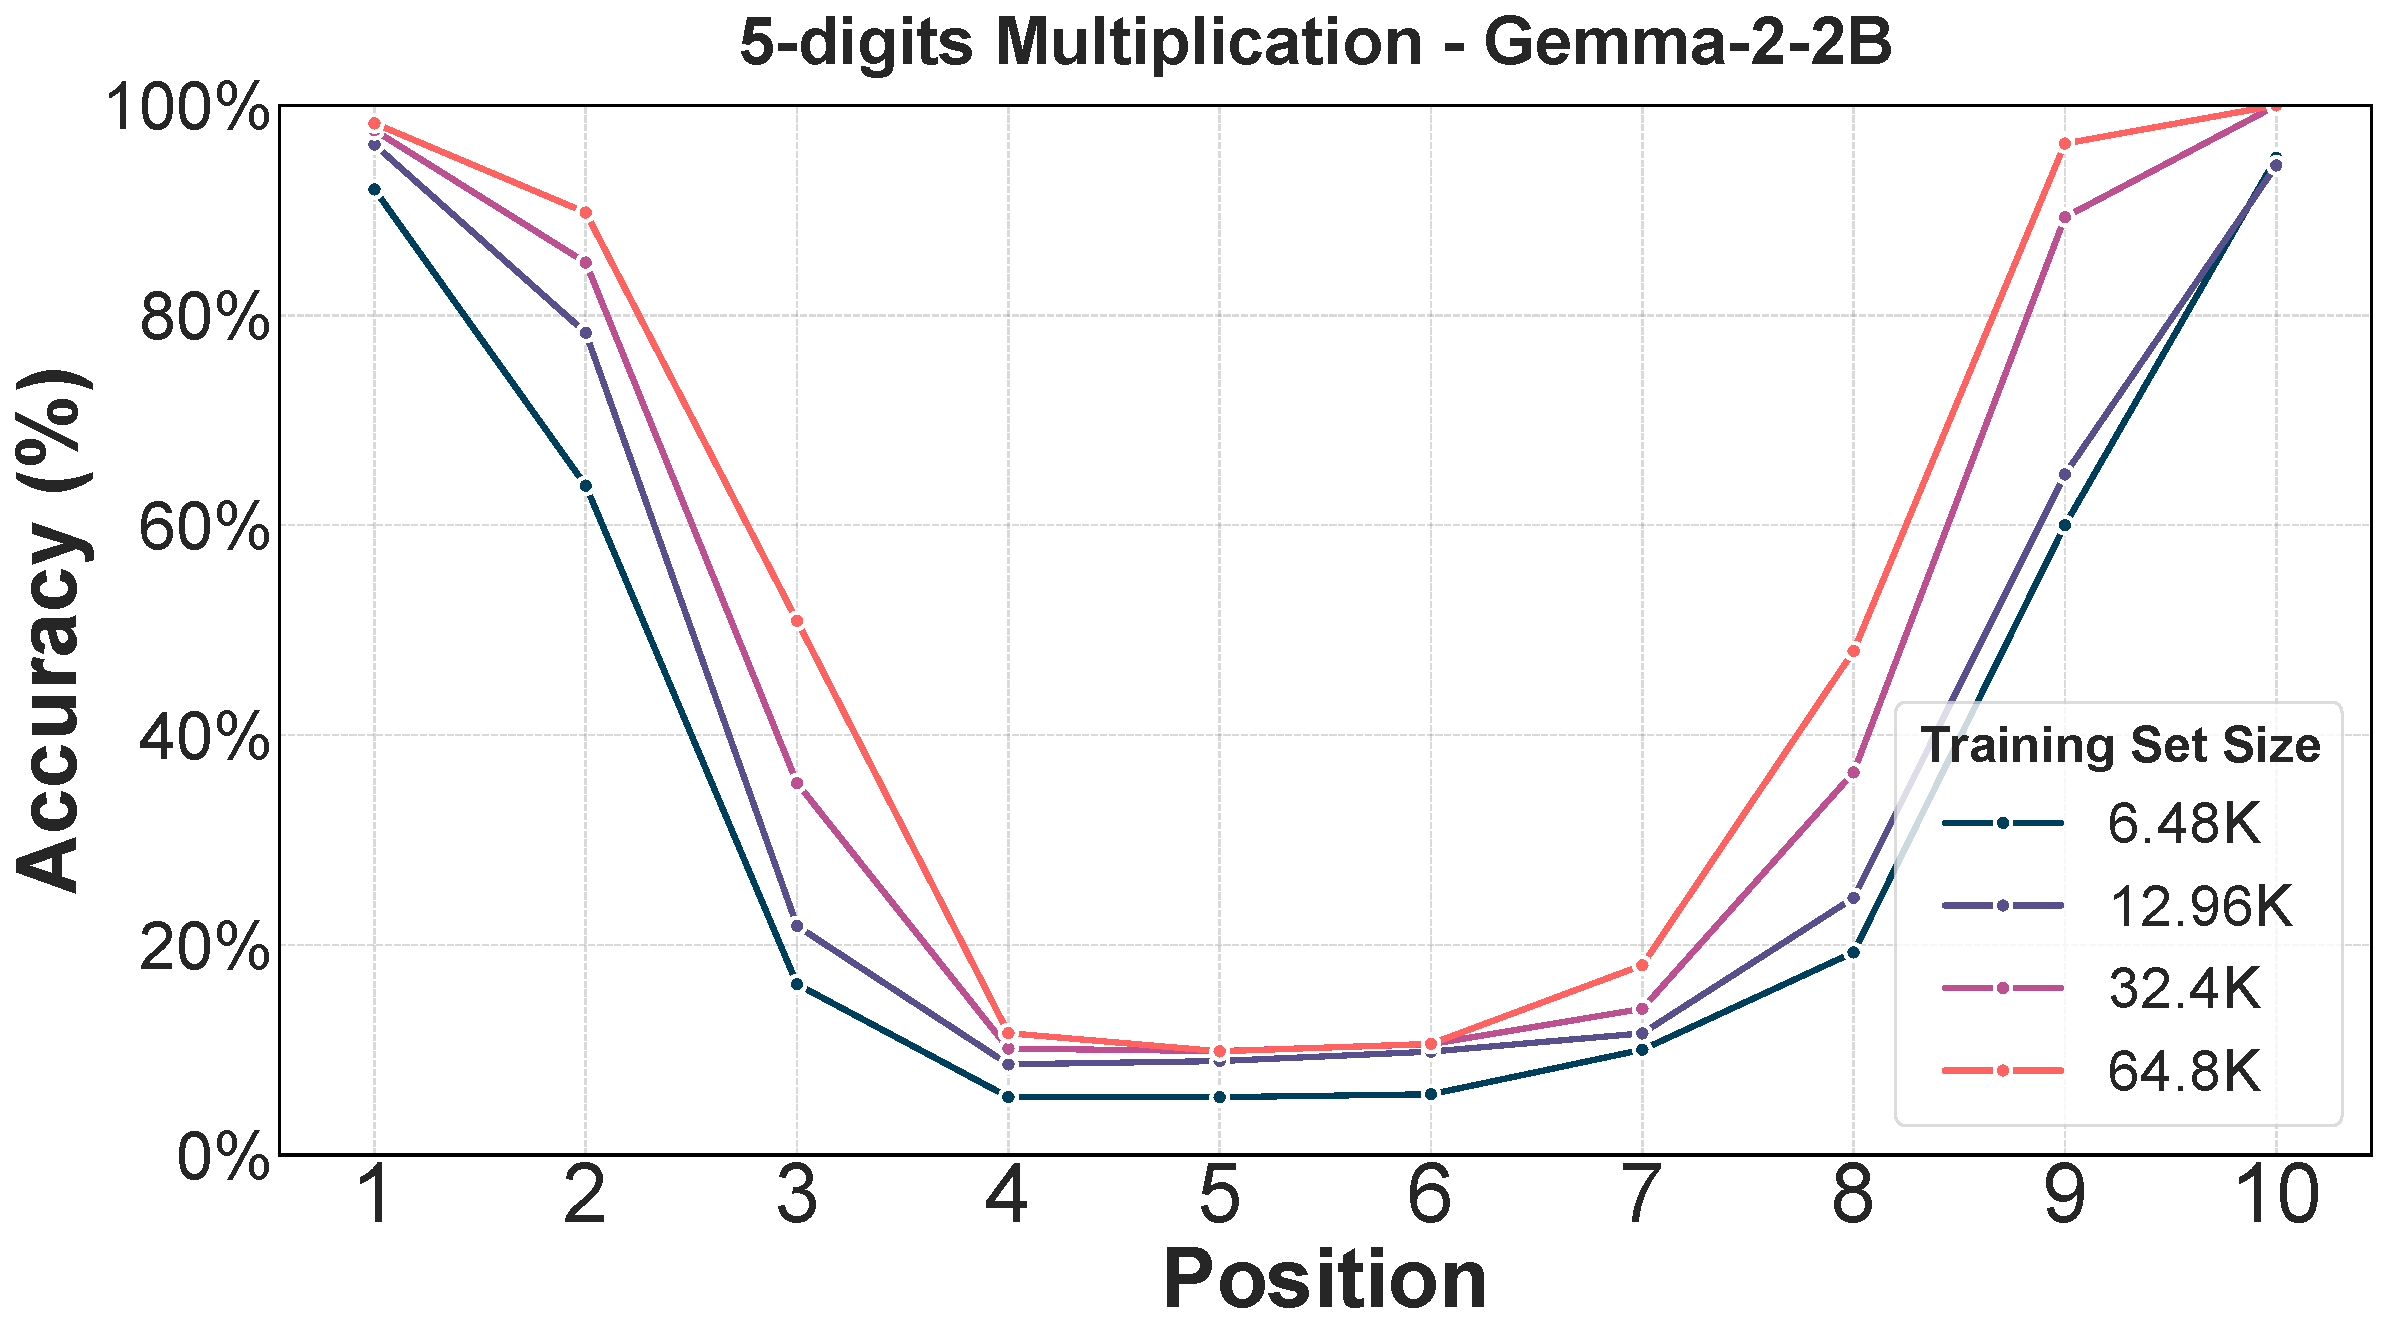
\includegraphics[width=0.33\linewidth]{figure/5x5_position_accuracy_chart_gemma1.pdf}
    \\\hspace{-0.4cm}
   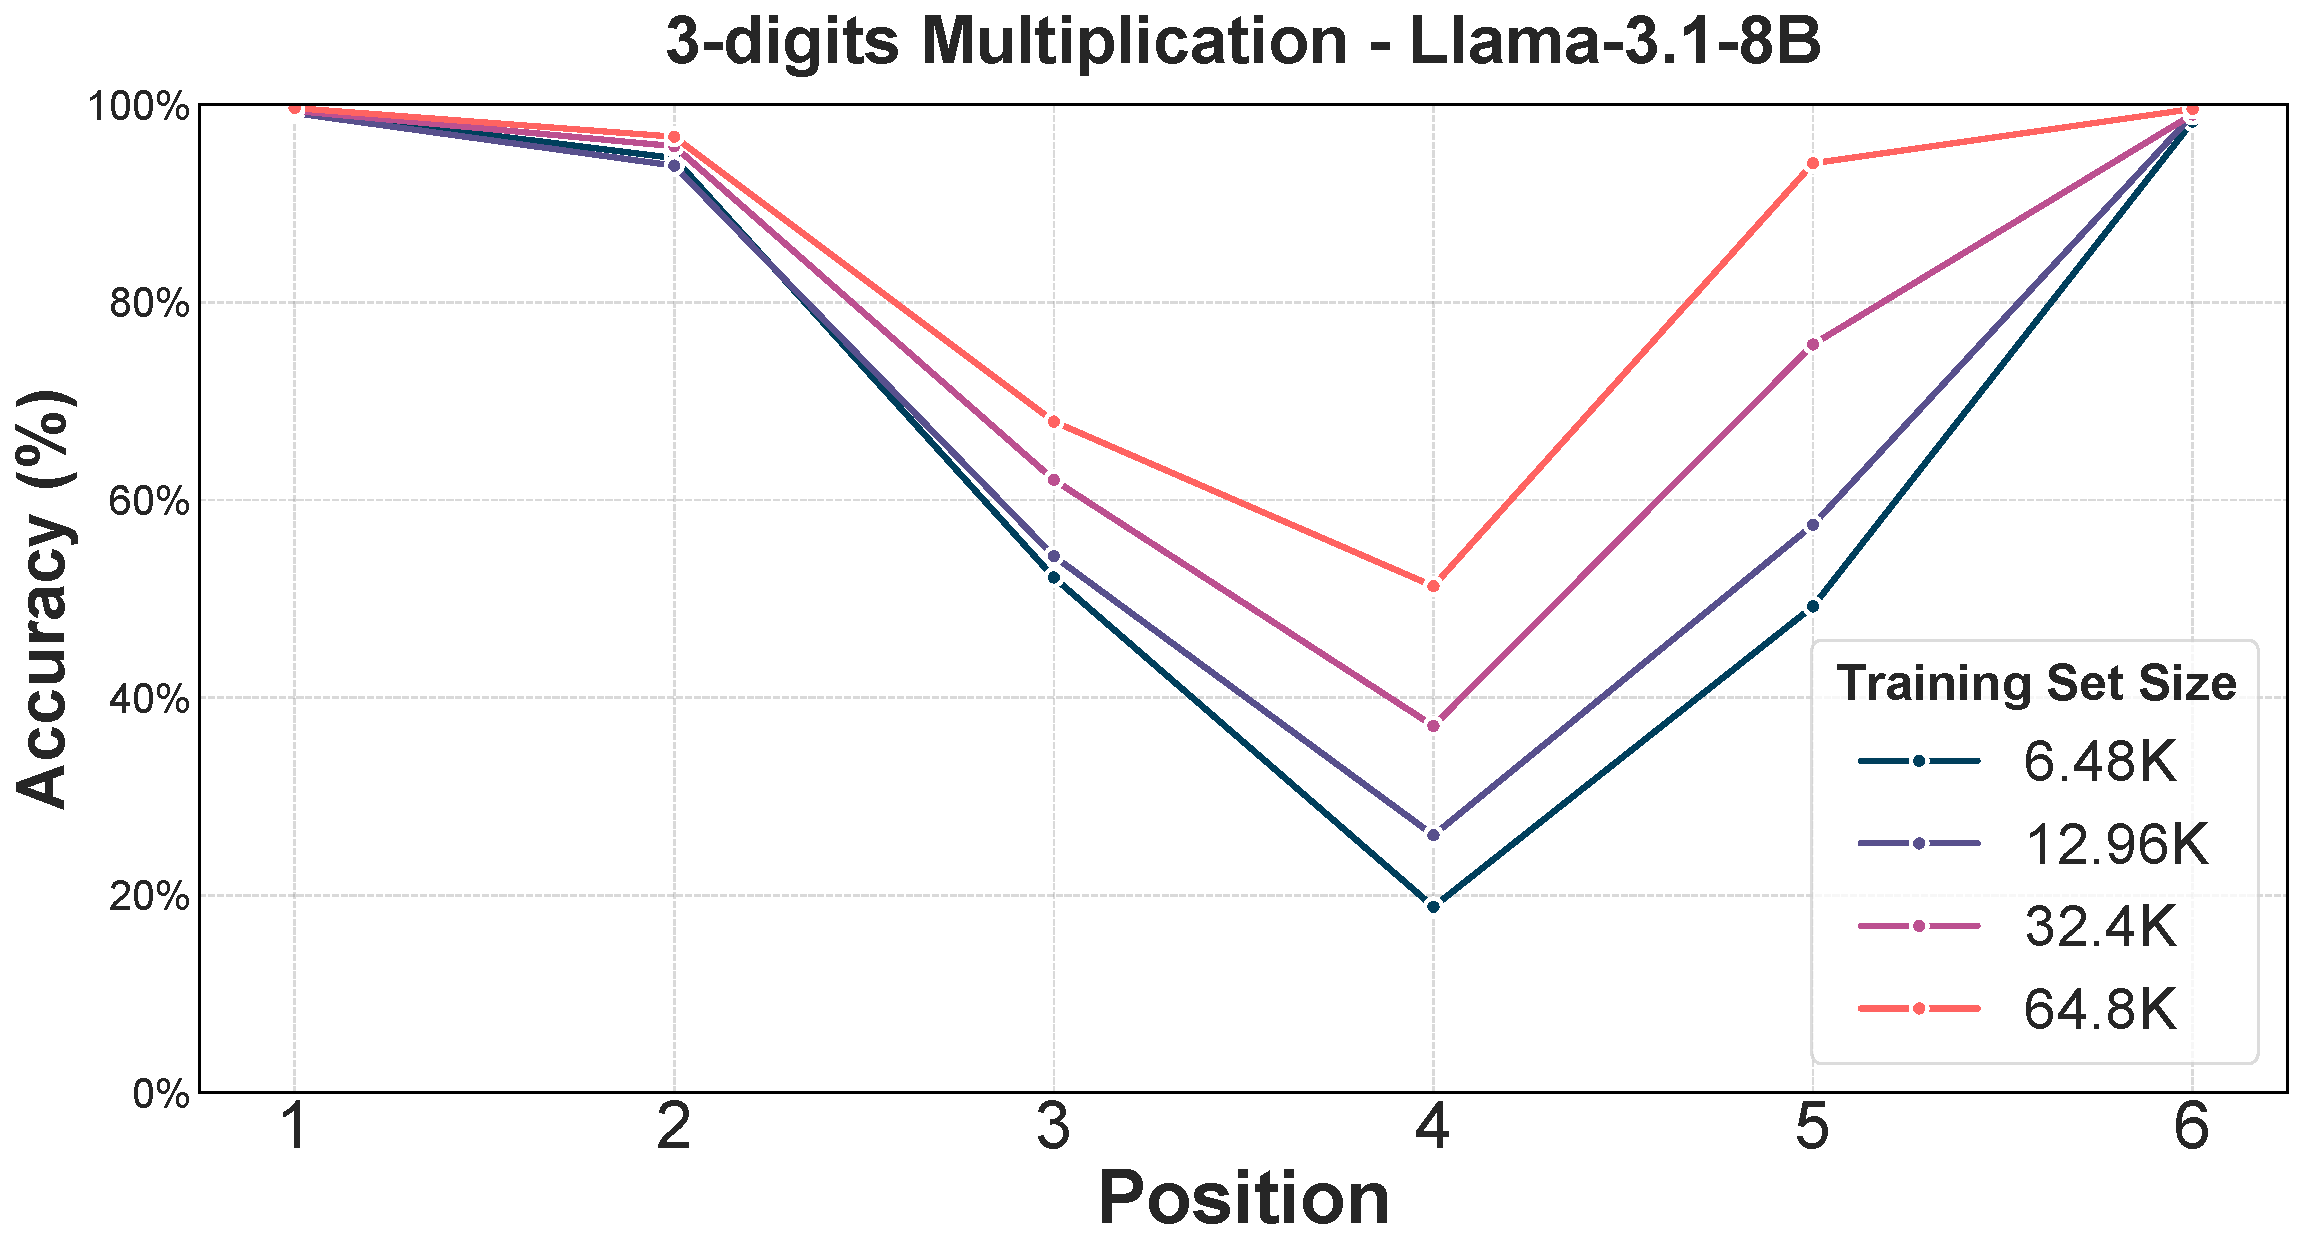
\includegraphics[width=0.33\linewidth]{figure/3x3_position_accuracy_chart-llama.pdf}
    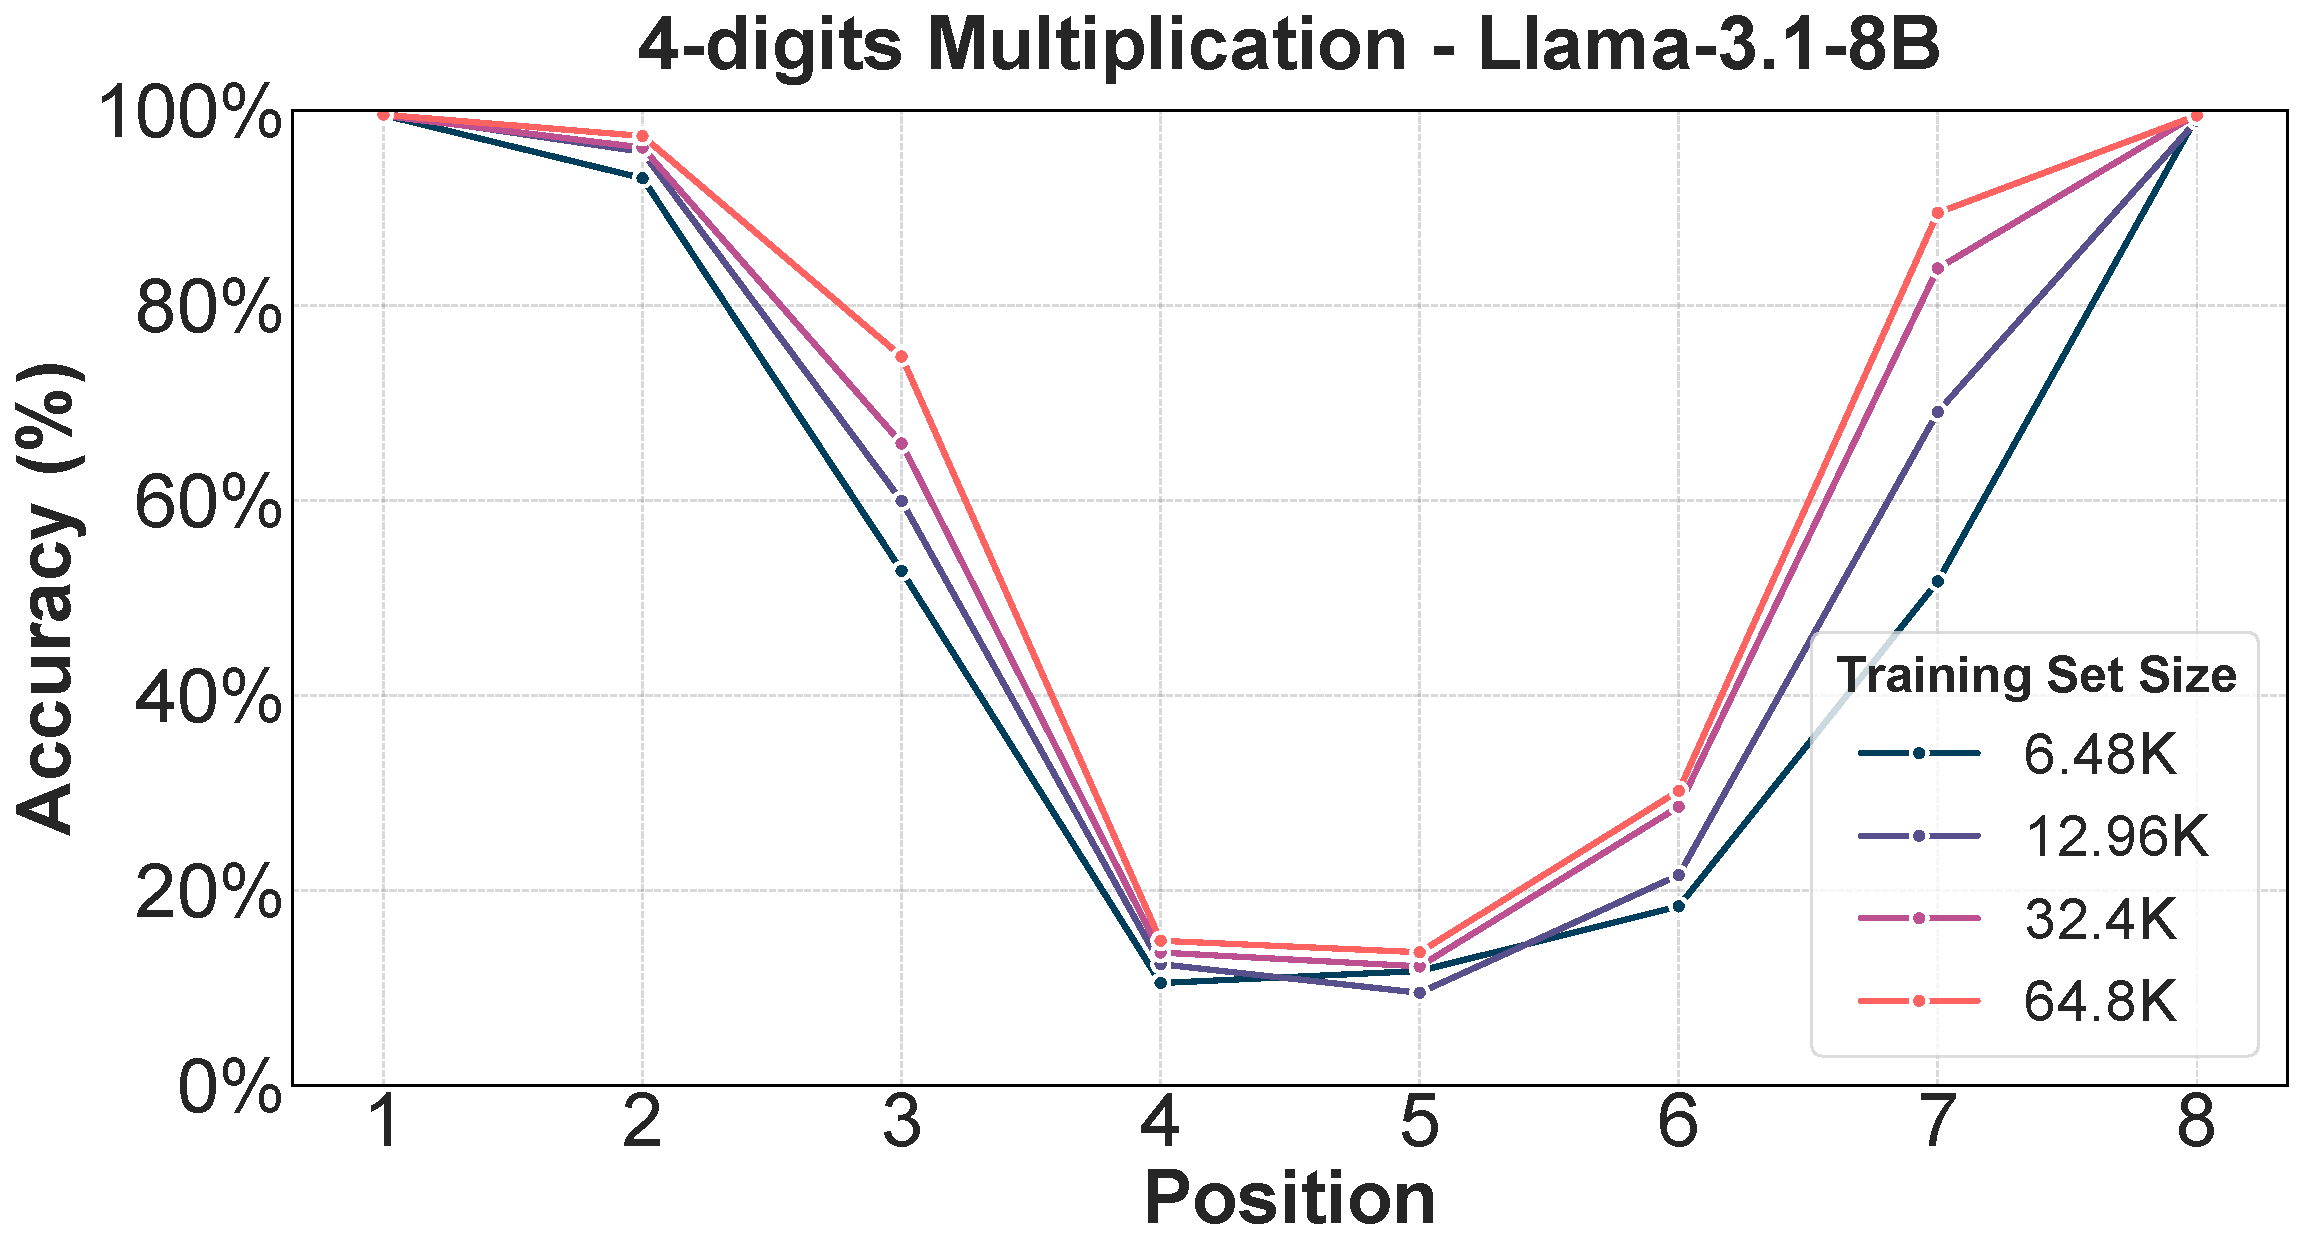
\includegraphics[width=0.33\linewidth]{figure/4x4_position_accuracy_chart-llama.pdf}
    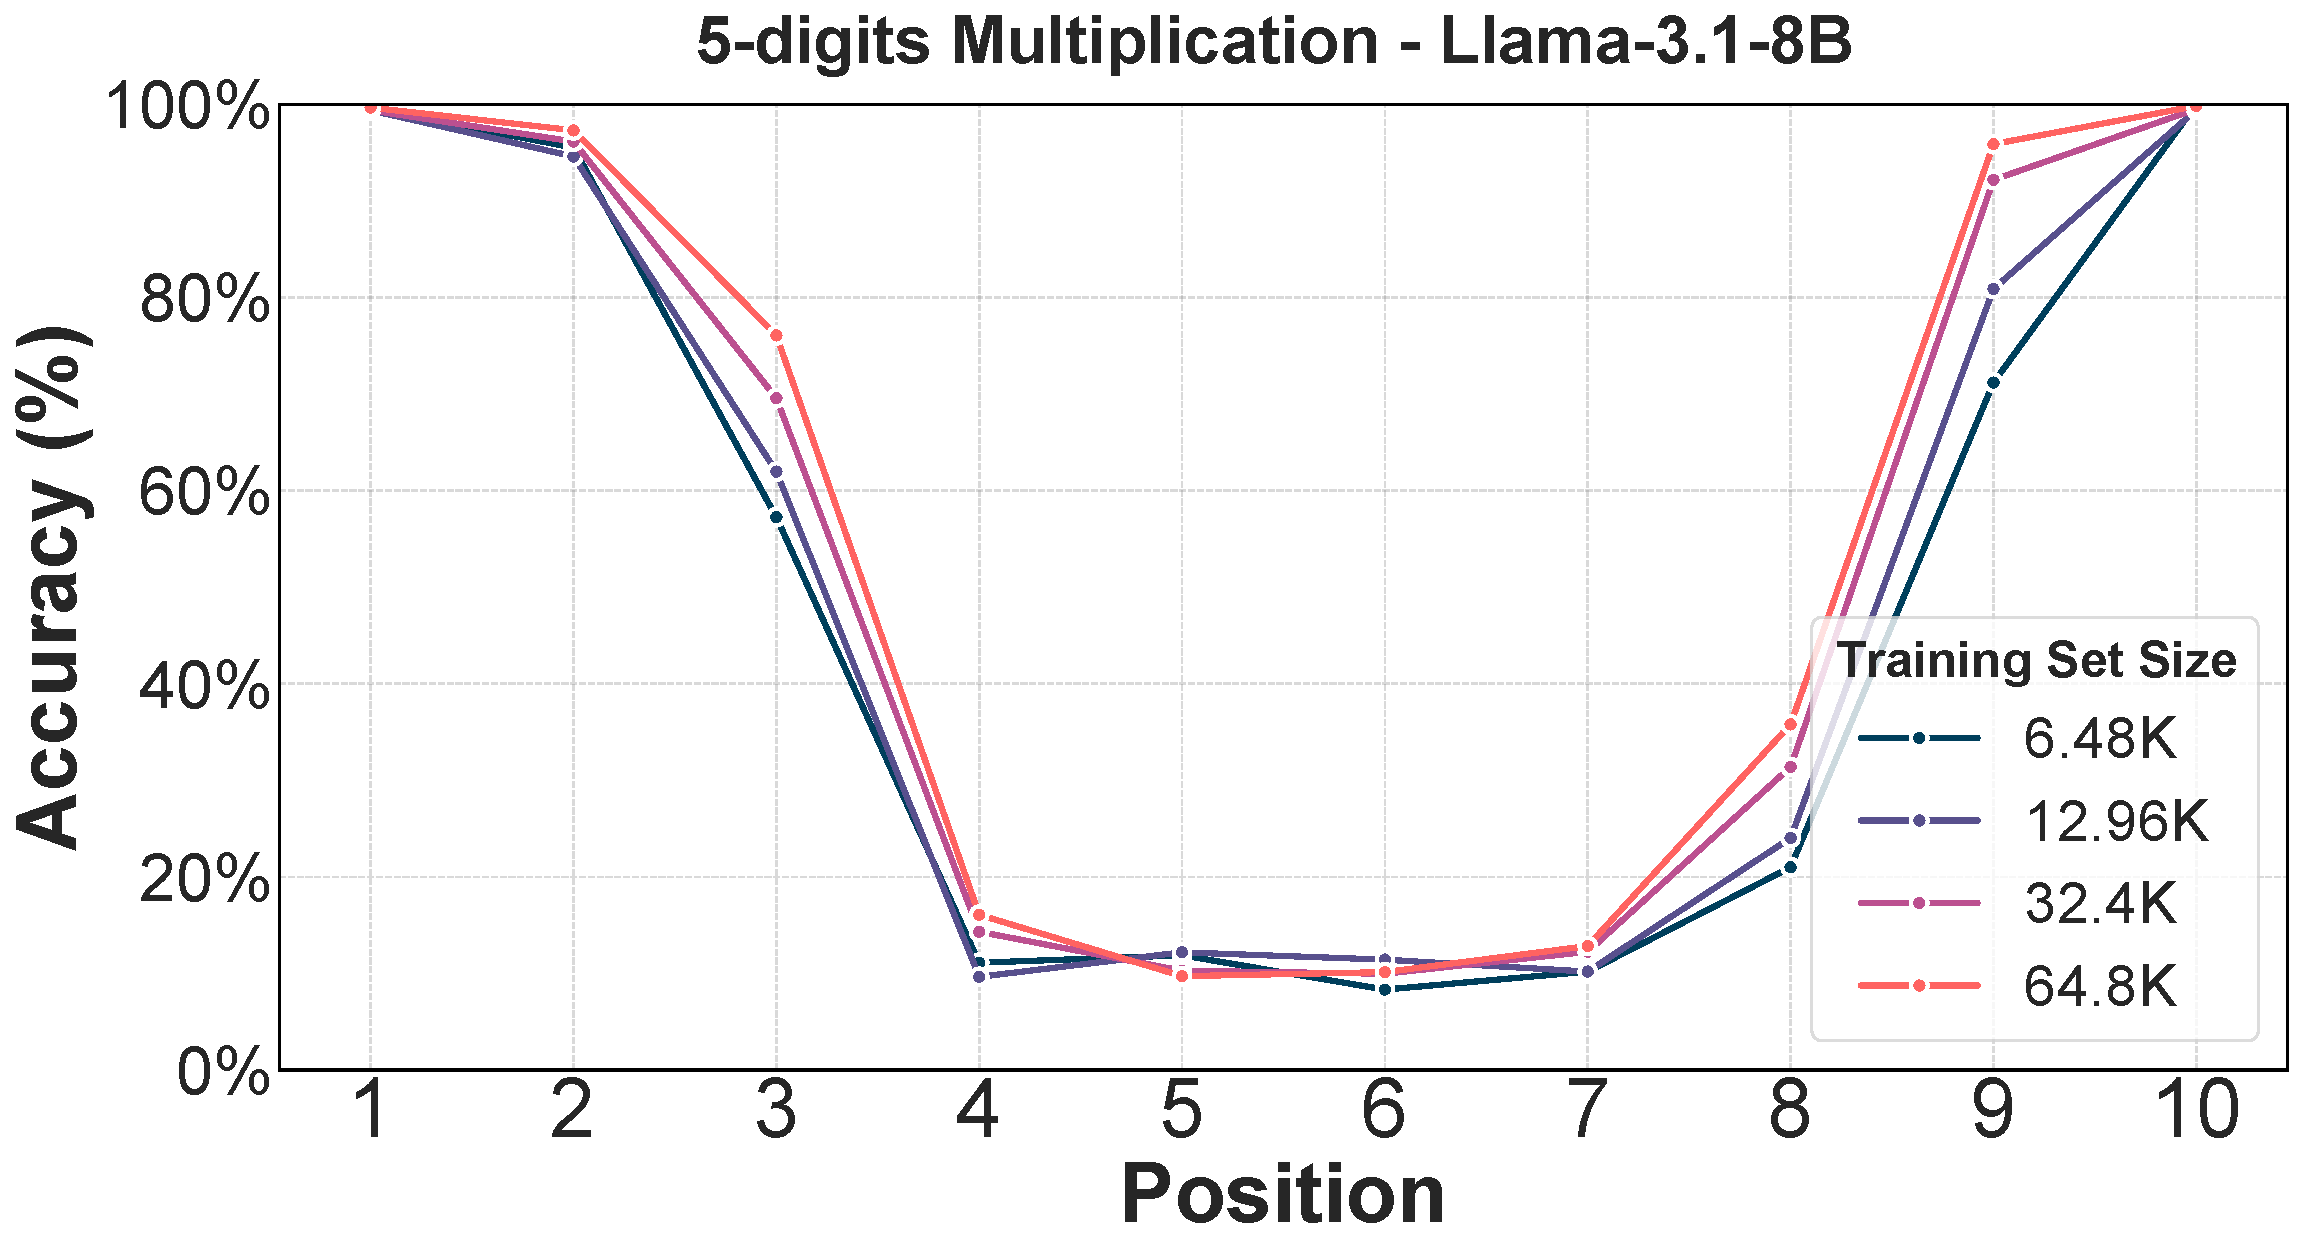
\includegraphics[width=0.33\linewidth]{figure/5x5_position_accuracy_chart_llama.pdf}

    \caption{Position-level Accuracy from Gemma-2-2B and Llama-3.1-8B.}
    \label{fig:position-level-acc}
    \vspace{-0.4cm}
\end{figure*}
\subsection{Subgroup Selection: Revealing Learning Dynamic in Arithmetic Learning}
\label{sec:subgroup-selection}
In the previous section, we established that subgroup space provides a basis for quantifying complexity in arithmetic tasks. However, the results mainly highlight insights at the end of learning (test accuracy after 12 epochs), leaving the learning dynamics less explored. Here, we investigate these dynamics by analyzing digit-level accuracy in model outputs, observing how LLMs select subgroups $S_n$ based on their performance across different positions.

\paragraph{Settings}
We maintain the same basic experimental settings as in the previous section to ensure the discussion remains within the same scope. We will train Gemma-2-2B and Llama-3.1-8B on four different dataset sizes (\(6.48K\), \(12.96K\), \(32.4K\), and \(64.8K\)). Our experiments cover multiplication tasks ranging from $3$-digit to $5$-digit numbers, with output digits from $6$ to $10$.
\paragraph{Position-level Accuracy are U-curve}
Figure~\ref{fig:position-level-acc} reveals a phenomenon overlooked in previous studies. Contrary to the common assumption that position-level accuracy decreases from right to left due to carryover effects and least-to-most significant digit calculations~\citep{lee2023teachingarithmeticsmalltransformers,zhangli2024reversenumberdecodingorder}, our results show a U-shaped accuracy curve in both Gemma-2-2B and Llama-3.1-8B models. Accuracy peaks at the beginning and end positions, exceeding $95\%$, with lower accuracy (\textasciitilde$10\%$) in the middle positions, especially in higher-digit multiplication (e.g., 4th/5th for 4-digit, 5th/6th for 5-digit).These results provide valuable insights, suggesting that the difficulty in learning multiplication is concentrated in the middle positions rather than at the beginning, which conceptually corresponds to the final steps of calculation.

\paragraph{Subgroup Selection via Quality}
We think that the U-curve occurs because the subgroup for middle digits has a lower subgroup quality \( Q(s) \) compared to the beginning and end digits. Given a subgroup \( s = ((\mathbb{A}, \mathbb{B}), \mathbb{C}) \), where \( \mathbb{C_{\text{mid}}} \) represents the middle digits, more digits from the operands are required to determine the value of \( \mathbb{C_{\text{mid}}} \) compared to representing digits at the beginning or end positions. This leads to a larger domain size \( |\mathcal{D}| \) when summing all candidates. Consequently, determining the value of \( \mathbb{C} \) becomes less certain, resulting in a lower \( Q(s) \). Specifically, when \( \mathbb{C} \) represents the last digit, its value can be fully determined by the least significant digits of the operands, which is not the case when \( \mathbb{C} \) represents a middle digit. For instance, in the case of 3-digit multiplication, it is relatively easy to identify the subgroup \( s = \{(\{A_1\}, \{B_1\}), \{C_1\}\} \) for learning the first digits or the subgroup \( s = \{(\{A_3\}, \{B_3\}), \{C_6\}\} \) for learning the last digits. This observation explains why the digits at the beginning or the end are easier to learn. It also reveals that LLMs fit arithmetic learning patterns following an easy-to-hard mechanism (from high \( Q(s) \) to low \( Q(s) \)), which demonstrates gradient descent in the "fastest" symbolic direction.


\section{Conclusions}
In this work, we investigate whether LLMs solve arithmetic tasks using partial products or operate as symbolic pattern matchers. Our findings confirm that LLMs do not rely on partial products but instead approach arithmetic purely symbolically. By breaking tasks into subgroups, we demonstrate that the difficulty in arithmetic learning can be attributed to subgroup complexity and selection. Our results emphasize the crucial role of label space entropy in understanding the convergence stage and the quality of subgroups for learning dynamics. Overall, at least in our setting, LLMs function as purely symbolic learners in arithmetic tasks. We encourage further research to explore more complex tasks from this perspective.
\section{Limitations}
In terms of limitations, one area our work does not currently address is the application of our framework to different chain-of-thought (CoT) methods~\citep{wei2023chainofthoughtpromptingelicitsreasoning,deng2024explicitcotimplicitcot}. While CoT has proven to be highly effective in arithmetic learning, particularly by decomposing overall difficulty into smaller, more manageable operations—thereby reducing subgroup complexity from exponential to linear—this aspect has not been explored in our study. Additionally, we have not applied our framework in a totally natural language-aware setting like GSM8K or MATH. Exploring how LLMs leverage their symbolic capabilities in such a context could provide deeper insights into their reasoning abilities, particularly in tasks that require structured, multi-step problem solving. These unexplored areas present significant opportunities for future research.
\section{Ethics Statement}
Our research primarily focuses on the symbolic learning capabilities of large language models in arithmetic tasks. As such, it does not involve the collection or use of any human data. No personal or sensitive information is handled or analyzed in this study. We acknowledge the potential biases inherent in the datasets used for model training and the limitations of relying on symbolic learning without fully understanding the underlying numerical or logical processes. The societal impact of increased reliance on LLMs for arithmetic tasks, including overconfidence in symbolic learning without full comprehension, warrants careful consideration. We advocate for transparent model evaluations and awareness of the limitations in deploying such models for critical decision-making.


\bibliography{custom}

\appendix

\section{Appendix}
\subsection{Training Detail}
\label{appendix:training-detail}
We carefully tuned the hyperparameters in our experiments. The learning rate for Gemma-2-2B was set to $1e-4$, while for Llama-3.1-8B it was $2e-4$. Both models used a warm-up of $5$ steps and a weight decay of $0.01$. We trained for $12$ epochs, splitting the dataset into $80\%$ for training, $10\%$ for validation, and $10\%$ for testing.  Evaluation was conducted at the end of each epoch, with checkpoints saved based on the best performance on the validation set. LoRA finetuning is used for both models with same setting, lora\_rank = $64$, lora\_alpha = $16$, lora\_dropout = $0$, and we enable rank stabalized lora~\citep{kalajdzievski2023rankstabilizationscalingfactor} during training. We use unsloth\footnote{Unsloth AI is at:~\url{https://unsloth.ai/}}\label{web:unsloth} to fasten our training process and vLLM~\citep{kwon2023efficient} to increase our inference process.
\begin{table*}[ht]
\centering
\small
\resizebox{\textwidth}{!}{
\begin{tabular}{llccccccc}
\toprule
& &\multicolumn{1}{c}{$C_1$} & \multicolumn{1}{c}{$C_2$}& \multicolumn{1}{c}{$C_3$}& \multicolumn{1}{c}{$C_4$}&\multicolumn{1}{c}{$C_5$} &\multicolumn{2}{c}{$\{C_j\}_{i=1}^{n}$} \\
 \cmidrule(lr){8-9} 
Task & Format & $H(\mathcal{L})$ & $H(\mathcal{L})$ &  $H(\mathcal{L})$ & $H(\mathcal{L})$ & $H(\mathcal{L})$ & $|\mathcal{L}|$ & $H(\mathcal{L})$ \\
\midrule
$f(a,b) = a+b$ & $A_1A_2+B_1B_2=C_1C_2C_3$ & $0.9710$ & $3.3215$ & $3.3219$ & $-$ & $-$ &$179$ &$7.2130$\\
$f(a,b) = a+b$ & What is $A_1A_2$ add $B_1B_2$? Answer: $C_1C_2C_3$   & $0.9649$ & $3.3215$ & $3.3219$ & $-$ & $-$ &$179$ &$7.2130$\\
$f(a,b) = a+b$ & fafr if $A_1A_2$ hfk $B_1B_2$? Ffhjar: $C_1C_2C_3$ & $3.3214$ & $3.3219$ & $-$ & $-$ & $-$ &$179$ &$7.2130$ \\
$f(a,b) = a+b$ & 3.123 34 $A_1A_2$ 461 $B_1B_2$? 952414: $C_1C_2C_3$ & $0.9280$ & $3.3214$ & $3.3219$ & $-$ & $-$ &$179$ &$7.2130$ \\
\midrule
$f(a,b) = a \times b$ & $A_1A_2 \times B_1B_2=C_1C_2C_3C_4C_5$  & $2.5811$ & $3.3202$ & $3.3151$ & $3.2235$ & $2.2227$ & $2621$ &$11.1172$\\
$f(a,b) = a \times b$ & What is $A_1A_2$ multiply $B_1B_2$? Answer: $C_1C_2C_3C_4$  & $2.8979$ & $3.3215$ & $3.3160$ & $3.0340$ & $-$ & $2621$ &$11.1172$\\
$f(a,b) = a \times b$ & fafr if $A_1A_2$ hfk $B_1B_2$? Ffhjar: $C_1C_2C_3C_4$ & $0.6873$ & $3.2173$ & $3.3215$ & $3.2964$ & $2.2227$ & $2621$ &$11.1172$ \\
$f(a,b) = a \times b$& 3.123 34 $A_1A_2$ 461 $B_1B_2$? 952414: $C_1C_2C_3C_4$ & $1.6030$ & $3.3020$ & $3.3204$ & $3.2234$ & $2.2227$ & $2621$ &$11.1172$\\
\bottomrule
\end{tabular}}
\caption{Label space statistics with different format perturbations. $H(\mathcal{L})$ represents the entropy of the space, and $|\mathcal{L}|$ is the size of the space. $\{C_j\}_{i=1}^{n}$ represents all possible output digits.}
\label{tab:format-perturbation}
\end{table*}
\begin{table}[t]
\vspace{-0.5cm}
\vspace{-0.2cm}
\centering
\small
\resizebox{0.5\textwidth}{!}{
\begin{tabular}{lccc}
\toprule
& \multicolumn{1}{c}{Format} & \multicolumn{1}{c}{Gemma-2-2B} & \multicolumn{1}{c}{Llama-3.1-8B} \\
\midrule
$f(a,b) = a+b$ & Natural Language& $-$ & $-$\\
$f(a,b) = a+b$  & Random String&$+0.1\%$ & $-0.2\%$ \\
$f(a,b) = a+b$  & Disturbed Digits &$-3.9\%$ & $-2.1\%$ \\
\midrule
$f(a,b) = a \times b$ & Natural Language& $-$ & $-$\\
$f(a,b) = a \times b$  & Random String&$+0.3\%$ & $-0.5\%$ \\
$f(a,b) = a \times b$  & Disturbed Digits &$-1.9\%$ & $-3.1\%$ \\
\bottomrule
\end{tabular}}
\caption{Test Accuracy difference $\Delta$ on perturbed addition and multiplication.}
\label{tab:data-format-results}
\end{table}
\subsection{Format Perturbations in Arithmetic Tasks}
\label{appendix:datA_format}
In this section, we apply three types of format perturbations to basic addition and multiplication tasks to evaluate the symbolic reasoning capabilities of large language models (LLMs). Our experiments utilize Gemma-2-2B and Llama-3.1-8B models. The primary objective of varying the input format is to investigate whether LLMs function as purely symbolic learners in arithmetic tasks. We consider the following three types of format perturbation in Table~\ref{tab:format-perturbation}:

\begin{enumerate}
    \item \textbf{Natural Language (NL):} Arithmetic expressions are converted into natural language statements. For example, the equation ``$3 + 5$'' becomes ``What is 3 times 5?''
    
    \item \textbf{Random String (RS):} Arithmetic expressions are first converted into natural language and then replaced with meaningless strings. Using the previous example, ``$3 + 5$'' might be transformed into ``flad kf 3 lfd 5?''
    
    \item \textbf{Disturbed Digits (DD):} Arithmetic expressions are initially converted into natural language and subsequently replaced with random digits. For instance, ``$3 + 5$'' could become ``65.1 44 3 4 5?'' This approach creates a counterfactual context for arithmetic tasks, increasing the difficulty for the models.
\end{enumerate}

By implementing these perturbations, we aim to assess the robustness of LLMs in handling arithmetic operations under varied and challenging input formats.


\paragraph{Results}
We examined the impact of three types of input format perturbations (Natural Language (NL), Random String (RS), and Disturbed Digits (DD)) on the arithmetic reasoning tasks for Gemma-2.2B and Llama-3.1-8B models. Table \ref{tab:data-format-results} shows that across both addition and multiplication tasks, the performance of the models remains largely unaffected by the perturbations when the label space is fixed. Specifically, there is only a marginal change in accuracy under the NL and RS formats, while the DD format causes minor fluctuations but does not significantly degrade performance. This demonstrates that LLMs can effectively handle various input perturbations as long as the output space remains consistent, suggesting their robustness in symbolic reasoning tasks despite superficial input variations.
\subsection{Mathematical Explanation of Diagnostic Sets for Multiplication Algorithms}
\label{appendix:diagnostiC_sets}
For the multiplication task involving two two-digit numbers formatted as $A_1A_2 \times B_1B_2 = C_1C_2C_3C_4$, we generate diagnostic test sets $\mathcal{P}$ for each algorithm to analyze and understand the partial computations involved. Below, we provide a mathematical explanation for the formulation of these diagnostic sets for each multiplication algorithm.
\subsubsection{Standard Multiplication}
In the standard multiplication algorithm, we multiply each digit of one number by each digit of the other number and sum the appropriately weighted results.

\textbf{Formulation:}
Let the two-digit numbers be expressed as:
\begin{align*}
a &= A_1A_2 = 10A_1 + A_2, \\
b &= B_1B_2 = 10B_1 + B_2.
\end{align*}

The product is:
\[
ab = (10A_1 + A_2)(10B_1 + B_2).
\]

Expanding, we get four partial products:
\[
ab = 100A_1B_1 + 10A_1B_2 + 10A_2B_1 + A_2B_2.
\]

\textbf{Diagnostic Set:}
\[
\mathcal{P}_{\text{std}} = \left\{ A_1 \times b,\ A_2 \times b,\ B_1 \times a,\ B_2 \times a \right\}.
\]

\textbf{Explanation:}

\begin{itemize}
\item $A_1 \times b$: Multiplying the tens digit of $a$ by the entire number $b$:
  \[
  A_1 \times b = A_1 \times (10B_1 + B_2) = 10A_1B_1 + A_1B_2.
  \]
  
\item $A_2 \times b$: Multiplying the units digit of $a$ by $b$:
  \[
  A_2 \times b = A_2 \times (10B_1 + B_2) = 10A_2B_1 + A_2B_2.
  \]
  
\item $B_1 \times a$: Multiplying the tens digit of $b$ by $a$:
  \[
  B_1 \times a = B_1 \times (10A_1 + A_2) = 10A_1B_1 + A_2B_1.
  \]
  
\item $B_2 \times a$: Multiplying the units digit of $b$ by $a$:
  \[
  B_2 \times a = B_2 \times (10A_1 + A_2) = 10A_1B_2 + A_2B_2.
  \]
\end{itemize}

Including these partial products in $\mathcal{P}_{\text{std}}$ captures all intermediary computations in the standard algorithm, facilitating a comprehensive diagnostic analysis.

\subsubsection{Repetitive Addition}

Repetitive addition interprets multiplication as adding one number to itself repeatedly.

\textbf{Diagnostic Set:}
\[
\mathcal{P}_{\text{ra}} = \left\{ \sum_{i=1}^{b} a,\ \sum_{j=1}^{a} b \right\}.
\]

\textbf{Explanation:}

\begin{itemize}
\item $\sum_{i=1}^{b} a$: Adding $a$ to itself $b$ times:
  \[
  \sum_{i=1}^{b} a = a + a + \dots + a \quad (b \text{ times}) = ab.
  \]
  
\item $\sum_{j=1}^{a} b$: Adding $b$ to itself $a$ times:
  \[
  \sum_{j=1}^{a} b = b + b + \dots + b \quad (a \text{ times}) = ab.
  \]
\end{itemize}
Both summations lead to the same product $ab$, and including them in $\mathcal{P}_{\text{ra}}$ allows for analyzing both repetitive addition paths in the algorithm.
\subsubsection{Lattice Method}
The lattice method (or grid method) organizes the multiplication of each digit pair in a grid and sums along diagonals.

\textbf{Diagnostic Set:}
\[
\mathcal{P}_{\text{lattice}} = \left\{ A_1 \times B_1,\ A_1 \times B_2,\ A_2 \times B_1,\ A_2 \times B_2 \right\}.
\]
\textbf{Explanation:}
\begin{itemize}
\item $A_1 \times B_1$: Tens digit of $a$ times tens digit of $b$.
\item $A_1 \times B_2$: Tens digit of $a$ times units digit of $b$.
\item $A_2 \times B_1$: Units digit of $a$ times tens digit of $b$.
\item $A_2 \times B_2$: Units digit of $a$ times units digit of $b$.
\end{itemize}
These products fill the cells of the lattice grid:
\[
\begin{array}{c|cc}
\toprule
& B_1 & B_2 \\
\midrule
A_1 & A_1B_1 & A_1B_2 \\
A_2 & A_2B_1 & A_2B_2 \\
\bottomrule
\end{array}
\]
Summing along the diagonals yields the final product. Including these partial products in $\mathcal{P}_{\text{lattice}}$ covers all the necessary computations in the lattice method.

\subsubsection{Egyptian Multiplication}

Egyptian multiplication involves doubling the multiplicand and adding specific results based on the binary representation of the multiplier.

\textbf{Diagnostic Set:}
\[
\mathcal{P}_{\text{egyptian}} = \left\{ 2^k \times a\ \middle|\ k = 0, 1, \dots, \left\lfloor \log_2 b \right\rfloor \right\}.
\]

\textbf{Explanation:}

\begin{itemize}
\item \textbf{Binary Representation of $b$:} Express $b$ as a sum of powers of two:
  \[
  b = \sum_{k=0}^{n} C_k 2^k,\quad C_k \in \{0,1\},\ n = \left\lfloor \log_2 b \right\rfloor.
  \]
  
\item \textbf{Doubling $a$:} Compute successive doublings of $a$:
  \[
  2^0 \times a,\ 2^1 \times a,\ \dots,\ 2^n \times a.
  \]
  
\item \textbf{Selection and Summation:} Identify which $2^k \times a$ correspond to $C_k = 1$ in $b$'s binary representation and sum them:
  \[
  ab = \sum_{k=0}^{n} C_k (2^k \times a).
  \]
\end{itemize}

Including all $2^k \times a$ up to $n$ in $\mathcal{P}_{\text{egyptian}}$ ensures that we have the necessary partial products for any $b$, allowing us to reconstruct $ab$ by selecting and summing the appropriate terms.

\textbf{Example:}

If $b = 13$, its binary representation is $1101$, so $b = 2^3 + 2^2 + 2^0$. The partial products are:
\begin{align*}
2^0 \times a &= a, \\
2^1 \times a &= 2a, \\
2^2 \times a &= 4a, \\
2^3 \times a &= 8a.
\end{align*}
Select $2^0 \times a$, $2^2 \times a$, and $2^3 \times a$ (since $C_0 = C_2 = C_3 = 1$) and sum:
\[
ab = a + 4a + 8a = 13a.
\]

By formulating the diagnostic sets $\mathcal{P}$ as above for each multiplication algorithm, we encapsulate all intermediary computational steps inherent to each method.

\end{document}
